\documentclass{article}
\usepackage{arxiv}

% Professional header setup
\renewcommand{\undertitle}{}
\renewcommand{\shorttitle}{}
\renewcommand{\headeright}{}

% Override arxiv.sty header with clean professional layout
\AtBeginDocument{
  \fancyhf{}
  \fancyhead[L]{\footnotesize\textit{Corrigibility as a Structural Precondition for DPI}}
  \fancyhead[R]{\footnotesize\textit{Aravind}}
  \fancyfoot[C]{\thepage}
  \renewcommand{\headrulewidth}{0.4pt}
}

% arXiv preprint format - packages loaded in dependency order
\usepackage{amsmath,amssymb,amsthm}
\usepackage{libertinust1math}        % Libertinus math (must follow amsmath)
\usepackage{graphicx}
\usepackage{booktabs}
\usepackage{array}
\usepackage{float}
\usepackage[inline]{enumitem}
\usepackage{authblk}

% These must come BEFORE hyperref
\usepackage{xcolor}
\usepackage{colortbl}
\usepackage{url}
\usepackage{natbib}

% Hyperref (must load before hyperxmp)
\usepackage[
    colorlinks=true,
    linkcolor=blue!70!black,
    citecolor=green!50!black,
    urlcolor=blue!60!black,
    bookmarks=true,
    pdfauthor={Anivar A Aravind (ORCID: 0009-0009-8995-0005)},
    pdftitle={Corrigibility as a Structural Precondition for Digital Public Infrastructure: A Cybernetic Framework},
    pdfsubject={Structural evaluation framework for Digital Public Infrastructure using cybernetics, commons governance, and free software principles. Proposes five tests (EXIT, CODE, AUDIT, GOVERN, FORK) to verify whether systems permit correction by those they affect.},
    pdfkeywords={%
        Digital Public Infrastructure, DPI, G20 DPI Framework, Infrastructure Governance, Public Infrastructure Accountability, %
        Corrigibility, Structural Accountability, Five Tests Framework, EXIT CODE AUDIT GOVERN FORK, %
        AI Alignment, AI Corrigibility, Learned Systems, Training Data Governance, AI Ethics, Machine Learning Accountability, %
        Cybernetics, Ashby Law, Requisite Variety, Feedback Control Systems, Control Theory, %
        Commons Governance, Ostrom Design Principles, Digital Commons, Infrastructure Commons, %
        Free Software, Open Source Governance, Forkability, Software Freedom, Four Freedoms, %
        Digital Rights, Digital Autonomy, Surveillance Infrastructure, Consent Architecture, %
        India Stack, Aadhaar, UPI, Pix, Open-washing, Safety-washing, %
        Constitutional Preconditions, Tech Law, Administrative Law, Proportionality Review%
    },
    pdfcreator={LaTeX with hyperref},
    pdfproducer={pdfTeX},
    pdflang={en}
]{hyperref}

% Hyperxmp for XMP metadata and CC0 license (must load after hyperref)
\usepackage{hyperxmp}
\hypersetup{
    pdfcopyright={This work is dedicated to the public domain under CC0 1.0 Universal.},
    pdflicenseurl={https://creativecommons.org/publicdomain/zero/1.0/},
    pdfcontacturl={https://anivar.net},
    pdfcontactemail={ping@anivar.net},
    pdfauthortitle={Independent Researcher},
    pdfmetalang={en},
    pdftype={Text}
}

% Force Author in PDF info dict using pdfTeX primitive
\makeatletter
\AtBeginDocument{%
  \ifx\pdfinfo\@undefined\else
    \pdfinfo{/Author (Anivar A Aravind \string(ORCID: 0009-0009-8995-0005\string))}%
  \fi
}
\makeatother
\urlstyle{same}
\usepackage{listings}
\usepackage{tikz}
\usetikzlibrary{shapes.geometric, arrows.meta, positioning, calc, fit, backgrounds, shadows.blur, decorations.pathreplacing}
\usepackage{pgfplots}
\pgfplotsset{compat=1.17}
\usepgfplotslibrary{fillbetween}
\usepackage{tcolorbox}
\usepackage{subcaption}
\usepackage{capt-of}

% JSON styling for schema listings
\lstdefinelanguage{json}{
    basicstyle=\ttfamily\scriptsize,
    showstringspaces=false,
    breaklines=true,
    frame=single,
    backgroundcolor=\color{gray!3},
    rulecolor=\color{gray!40},
    framesep=3pt,
    xleftmargin=3pt,
    xrightmargin=3pt,
    literate=
      *{:}{{{\color{gray!70}:}}}{1}
       {,}{{{\color{gray!70},}}}{1}
       {\{}{{{\color{codecolor}\{}}}{1}
       {\}}{{{\color{codecolor}\}}}}{1}
       {[}{{{\color{auditcolor}[}}}{1}
       {]}{{{\color{auditcolor}]}}}{1}
       {"}{{{\color{governcolor}"}}}{1},
    morestring=[b]",
    stringstyle=\color{blue!60!black},
}

% Define colors for test names
\definecolor{exitcolor}{HTML}{06B6D4}
\definecolor{codecolor}{HTML}{3B82F6}
\definecolor{auditcolor}{HTML}{A855F7}
\definecolor{governcolor}{HTML}{F59E0B}
\definecolor{forkcolor}{HTML}{F472B6}

% Theorem environments
\newtheorem{definition}{Definition}
\newtheorem{proposition}{Proposition}
\newtheorem{claim}{Claim}
\newtheorem{theorem}{Theorem}
\newtheorem{condition}{Condition}
\newtheorem{corollary}{Corollary}

\title{Corrigibility as a Structural Precondition for Digital Public Infrastructure: A Cybernetic Framework}

\author[1]{Anivar A Aravind\thanks{Corresponding author: \href{https://anivar.net}{anivar.net} · \texttt{ping@anivar.net} · ORCID: \href{https://orcid.org/0009-0009-8995-0005}{0009-0009-8995-0005}}}
\affil[1]{Independent Researcher}

\date{January 2026}

\begin{document}

\maketitle

\begin{abstract}
\textbf{Digital Public Infrastructure (DPI) operates at the scale of populations.} Systems governing identity, payment, and data exchange effectively constitute a new administrative state. While international definitions from the G20 and United Nations articulate normative aspirations (that systems \textit{should} be open, inclusive, and safe), they largely lack the structural requirements to verify these attributes.

This paper proposes a formal evaluation framework based on \textbf{corrigibility}: the structural capacity of those affected by a system to detect error, signal harm, and trigger correction. We synthesize necessary conditions from three traditions: cybernetics (Ashby's Law of Requisite Variety), commons governance (Ostrom's design principles), and free software (Stallman's four freedoms). The resulting framework identifies five non-negotiable properties: \textbf{Reversibility, Inspectability, Verification, Constraint, and Reproduction}. We demonstrate that a failure in any single dimension breaks the feedback loop required for system stability. Furthermore, we extend this framework to learned systems (AI) and establish evidentiary standards for distinguishing authentic governance from performative compliance. The framework is released under CC0 public domain.
\end{abstract}

\section{Introduction}

Digital Public Infrastructure is not merely a collection of software stacks; it is the encoding of political arrangements into technical artifacts \citep{winner1980}. Access to essential survival services (food distribution, banking, healthcare, mobility) is increasingly mediated through these systems. Because these systems apply fixed rules to the infinite variety of human life, they will inevitably misclassify, exclude, or fail specific users. This is not a malfunction; it is a mathematical certainty when finite rule sets encounter human diversity.

The critical question for a digital polity is not whether errors occur, but whether the architecture permits those affected to \textbf{detect, correct, and reverse} them before harm becomes permanent.

Current policy discourse defines DPI through aspirational language. The G20 New Delhi Declaration (2023) and the UN/UNDP framework \citep{undp} describe systems that ``should be secure'' or ``can be built on open standards.'' These definitions exclude almost nothing. They articulate intent, not condition. Under such broad definitions, a system that traps users in a coercive loop can be labeled ``public infrastructure'' simply because it operates at scale.

This paper defines corrigibility not as a moral preference, but as a structural property essential for stability. We argue that \textbf{unverifiable constraint is structurally indistinguishable from absolute operator control.} Therefore, public legitimacy requires more than policy assertions; it requires a cryptographic chain of custody and a verifiable capacity for correction.

\paragraph{Paper Structure.} Section~\ref{sec:problem} diagnoses why current DPI definitions fail. Section~\ref{sec:theory} establishes the theoretical foundations from cybernetics, commons governance, and free software. Section~\ref{sec:tests} derives the five structural tests. Section~\ref{sec:dynamics} analyzes temporal dynamics and the correction velocity inequality. Section~\ref{sec:learned} extends the framework to AI systems. Section~\ref{sec:diagnosis} provides empirical evaluation of existing infrastructure. Section~\ref{sec:discussion} addresses implications, including essential services and agentic scaling. The appendices formalize the control-theoretic proofs and provide machine-readable schemas for automated assessment.

\paragraph{Key Terms.}
\begin{description}[style=nextline, leftmargin=1.5em, font=\normalfont\bfseries]
\item[Corrigibility] The structural capacity of those affected by a system to detect error, signal harm, and trigger correction. Not a moral preference but a stability requirement.
\item[Requisite Variety] Ashby's Law: a controller must have at least as many states as the system it regulates. Applied to DPI: governance mechanisms must match population diversity.
\item[Learned Systems] Infrastructure where behavior is determined by parameters learned from data (AI/ML) rather than explicit code logic.
\item[EXIT] Test 1: Reversibility of participation without prohibitive penalty.
\item[CODE] Test 2: Inspectability of system logic by affected parties.
\item[AUDIT] Test 3: Independent verification of correct operation.
\item[GOVERN] Test 4: Binding constraint that users can enforce, not advisory.
\item[FORK] Test 5: Capacity to reproduce infrastructure independently.
\item[Correction Velocity] Rate at which errors can be corrected; must exceed error accumulation rate for stability.
\item[GDoS] Governance Denial of Service: when agent interaction volume exceeds governance capacity.
\item[Open-washing] Claiming openness through partial compliance while retaining structural control.
\item[DID-washing] Using decentralized identifiers while maintaining centralized governance.
\item[Human Friction Buffer] The hidden subsidy where humans absorb system failures through delay and workaround, masking architectural incorrigibility.
\end{description}

\section{The Problem: Definitions Without Structure}
\label{sec:problem}

The accepted definitions of Digital Public Infrastructure share a common defect: they describe desired outcomes without specifying the architectural preconditions required to achieve them. The standard formulation (that DPI is a set of ``shared digital systems'' built on ``open standards'' \citep{g20}) leaves open four distinct vectors for capture.

First, \textbf{Open Standards are not Open Execution.} A proprietary system can speak a standard language (like a browser displaying HTML) while remaining entirely opaque in its internal logic. The interface is public; the machine is private. (Addressed by the \textbf{CODE} test, Section~\ref{sec:tests}.)

Second, \textbf{Legal Frameworks do not guarantee Technical Rights.} A system that requires a court order to correct a database error effectively denies correction to the majority of its users. Legal remedy operates on bureaucratic time; infrastructure operates on digital time. (Addressed by the correction velocity inequality, Section~\ref{sec:dynamics}.)

Third, \textbf{Aspiration is not Compliance.} Definitions that rely on what a system ``can'' do or ``should'' be offer no resistance to authoritarian drift. Modal language creates no enforceable constraint. (Addressed by the \textbf{GOVERN} test, Section~\ref{sec:tests}.)

Fourth, \textbf{Scale is not Accountability.} A system that serves a billion users achieves universality, but universal deployment does not confer public legitimacy. Population-scale operation may simply mean population-scale capture. The ``public'' in such definitions refers to the number of subjects, not the structure of control. (Addressed by the essential services problem, Section~\ref{sec:discussion}.)

Without hard structural requirements, ``Public'' becomes a mere descriptor of scale rather than a mode of accountability. Just as classification systems become invisible as they gain acceptance \citep{bowker1999}, incorrigible infrastructure recedes into the background, becoming unchallengeable precisely as it becomes essential. This danger is acute in the transition to AI-mediated governance, where ``Infrastructure'' begins to make probabilistic judgments rather than deterministic records.

\section{Theoretical Foundations}
\label{sec:theory}

This framework does not invent new ethical categories. Instead, it triangulates a single structural requirement from three independent intellectual traditions. Whether viewed through physics, political economy, or code, the stability of a system depends on the capacity of its subjects to provide corrective feedback.

\subsection{Cybernetics and Requisite Variety}

In cybernetics, the relationship between a controller and its environment is governed by Ashby's Law of Requisite Variety \citep{ashby1956}. The law states that for a system to be stable, the number of control states must meet or exceed the number of environmental states:

\begin{equation}
V(\text{controller}) \geq V(\text{disturbance})
\end{equation}

In DPI, the ``disturbance'' is the boundless diversity of the human population. No pre-programmed rule set can match this variety. Stability, therefore, relies on feedback channels that transmit error signals from the population back into the system's behavior. If these channels (specifically the ability to exit or correct) are blocked, the controller's variety effectively collapses. The system loses the capacity to regulate its own impact, leading inevitably to volatility or oppression.

\subsection{The Commons and Constitutional Constraint}

Elinor Ostrom's work on commons governance \citep{ostrom1990} establishes that sustainable systems require monitors who are accountable to the users and collective-choice arrangements that allow users to modify the rules. A system in which rule-making is the exclusive preserve of the operator acts as an enclosure, not a commons.

Critically, Ostrom identifies that governance is not merely about access; it is about graduated sanctions and low-cost conflict resolution. Applied to digital infrastructure, this implies that users must possess \textbf{Constitutive Power}: the ability to set binding limits on the system's behavior. If a system's constraints are merely advisory or can be overridden by the operator at will, the system is fundamentally ungoverned.

\subsection{Free Software and the Right to Reproduce}

The Free Software movement \citep{stallman2002} contributes the mechanical means of enforcement. Stallman's ``Four Freedoms'' are often misread as a philosophy of sharing, but they are functionally a philosophy of power. The freedom to study (Inspectability) ensures power is visible; the freedoms to modify and distribute (Reproduction) ensure that power is not a monopoly.

This tradition clarifies that openness is not a passive property (reading code) but an active one (forking infrastructure). Transparency without the power to act on it is voyeurism. The ability to reproduce the system independent of its original steward is the only ultimate check against operator capture.

\section{The Structural Conditions of Corrigibility}
\label{sec:tests}

We define corrigibility as the existence of specific mechanical capabilities that allow the subjects of a system to maintain control over it. Digital Public Infrastructure cannot rely on intent or policy to guarantee this property; it requires a specific architecture.

These capabilities form a hierarchy of defense. If a system lacks any single capability, the feedback loop breaks. Such a system becomes structurally indistinguishable from a monopoly exercising absolute control.

\subsection{Test 1: EXIT (Reversibility of Participation)}

The foundational condition of any corrigible system is the \textbf{Reversibility of Participation}. Irrevocable consent functions structurally as conscription. For an infrastructure to operate as a public utility rather than a coercive instrument, users must possess the capacity to withdraw from it without incurring disproportionate penalty or material exclusion.

In practice, many systems operate as a ratchet. They are easy to enter but functional imperatives make them impossible to leave. \textbf{Aadhaar} exemplifies this failure: opting out results in exclusion from banking, food rations, and mobile connectivity. When a system becomes a prerequisite for existence, refusal acts as self-immolation rather than feedback. \textbf{UPI} partially mitigates this because cash remains legal tender, but network effects increasingly marginalize non-participants. \textbf{Linux}, by contrast, imposes no survival penalty: a user can migrate to BSD or Windows without losing access to essential services.

From a cybernetic perspective, EXIT constitutes the primary negative feedback loop. Blocking this channel silences the user's error signal. This blockade overloads the political layer with demands that the technical layer has suppressed.

This dynamic was formalized by Hirschman \citep{hirschman1970} in his analysis of organizational decline. Hirschman distinguished two correction mechanisms: exit (withdrawal from participation) and voice (attempts to change the system from within). His central finding is that these mechanisms exist in productive tension, not as substitutes.

Exit, in Hirschman's formulation, is ``neat,'' ``impersonal,'' and ``indirect'': one either exits or one does not. This binary quality makes exit a high-bandwidth error signal. When users leave, the system receives unambiguous information that something has failed. Voice, by contrast, is costly and conditioned on the influence and bargaining power that participants can bring to bear. Voice is gradual, political, and requires sustained effort.

Critically, Hirschman demonstrated that exit without voice produces abandonment rather than correction: quality-conscious users flee rather than fight. But voice without exit produces capture: complaints become cosmetic (see Section~\ref{subsec:grievance}) because the system faces no credible threat of user departure. The effectiveness of voice depends on the credibility of exit.

This framework illuminates why mandatory enrollment is structurally pathological. By eliminating exit, a system does not merely suppress one feedback channel. It degrades voice itself. When citizens cannot leave, their complaints lack credibility. The operator can absorb infinite grievance without modifying system behavior ($\partial S / \partial G = 0$). Hirschman's insight formalizes what cybernetics predicts: blocking the error signal does not eliminate the error; it eliminates the system's capacity to respond.

\subsection{Test 2: CODE (Inspectability of Logic)}

Users who cannot leave a system must possess the ability to inspect it. \textbf{Inspectability of Logic} requires that the rules determining outcomes are visible to those they govern. Power in a digital system resides in execution. Lessig \citep{lessig2006} established that software architecture functions as regulation: code ``determines what people can or cannot do in the first place,'' unlike legal regulation which sets rules for behavior and retroactively punishes non-compliance. This is regulation without appeal. If the execution path remains hidden, that power is absolute; it is not merely unaccountable but structurally unobservable to those it governs.

Transparency specifications or open standards are insufficient if the executing artifact remains a black box. \textbf{Aadhaar's} CIDR (Central Identities Data Repository) is proprietary: the matching algorithm that determines identity cannot be examined. \textbf{UPI} publishes API specifications, but the NPCI switching logic remains closed. \textbf{Let's Encrypt} demonstrates the alternative: its CA software is fully open source, allowing anyone to audit the certificate issuance logic that secures web traffic. For learned systems, the challenge intensifies. \textbf{Llama} publishes inference weights but withholds training data composition and RLHF preferences. This is spec-as-source: you can run the model but cannot understand why it produces specific outputs.

\subsection{Test 3: AUDIT (Independent Verification)}

While inspection enables understanding, \textbf{Independent Verification} enables truth. This functions as the sensor in the cybernetic feedback loop. A system is verifiable only if external, permissionless actors can test its behavior, measure its error rates, and document its failure modes within production environments.

Incorrigible systems typically capture this function. \textbf{UPI} permits RBI regulatory audits, but transaction-level verification requires NPCI authorization; independent researchers cannot measure failure rates or dispute resolution times. \textbf{Open-weights AI models} (Llama, Qwen, DeepSeek) selectively publish red-teaming results while blocking independent adversarial testing at scale. \textbf{Bitcoin} provides the counter-model: every transaction is independently verifiable by any node, and consensus is cryptographic proof. Similarly, \textbf{Let's Encrypt} publishes Certificate Transparency logs, making every issued certificate publicly auditable in real time.

The structural function of opacity is sensor failure. A system whose error rates cannot be independently measured cannot be regulated. The controller receives no signal about divergence from intended behavior. Under Ashby's Law, such a system will drift until external forces impose correction. Those forces, operating outside the technical loop, will impose correction through channels the system cannot anticipate or absorb. \citet{pasquale2015} describes this as a ``one-way mirror'' relationship, but the cybernetic translation is precise: asymmetric observability breaks the feedback loop at the sensing stage.

\subsection{Test 4: GOVERN (Constitutive Constraint)}

Verification identifies the error, while \textbf{Constitutive Constraint} enforces the correction. This framework distinguishes structural governance from administrative functions like consultation, multi-stakeholder meetings, or feedback forms.

Governance exists only when binding constraints limit system behavior in ways the operator cannot override. \textbf{Aadhaar} is governed by UIDAI fiat: the same entity that operates the system sets its rules. \textbf{UPI} has NPCI governance, but NPCI is majority-owned by participating banks, creating structural conflicts. \textbf{Let's Encrypt} shows what binding constraint looks like: the ISRG charter legally binds the organization to its public benefit mission, with community board representation. \textbf{Bitcoin's} BIP process demonstrates governance through proven fork history; contentious changes have been rejected by the network, proving the community can override developer intent. \textbf{PostgreSQL's} contributor agreement prevents any single entity from capturing the project.

\subsubsection{The Post-Execution Fallacy}
A critical failure in modern policy involves relying on exogenous or post-hoc remedies to substitute for structural constraints. Mechanisms such as courts, ombudsmen, and grievance redressal officers operate on ``bureaucratic time,'' measured in months or years. Infrastructure operates on ``digital time,'' measured in milliseconds. A system that executes a harmful action, such as wrongful deletion of a beneficiary, and relies on a court order to reverse it six months later is structurally ungoverned for that duration. True governance must function within the system's execution loop to block prohibited states before they manifest.

Consequently, claims of governance must be evidentiary rather than declarative. They require a signed cryptographic chain of custody linking the operator's authority to an external, non-overrideable instrument.

\subsubsection{Strategic Openness vs Structural Accountability}

Open artifacts do not guarantee open governance. Both market-gardener and state-architect doctrines deploy openness instrumentally: releasing code or weights for adoption while retaining control over training, direction, and future development. Llama's weights are public; Meta controls alignment decisions. Android's AOSP is open; Google controls Play Services. This pattern (asymmetric openness) releases the artifact while closing the correction loop.

The GOVERN test requires bidirectional accountability: not merely that citizens can observe the system, but that they can correct it. Openness can be weaponized. Strategic openness maximizes visibility into users while minimizing user power over the system. This is the inverse of corrigibility: surveillance, not governance. True corrigibility requires the correction loop be open, not merely the artifacts. A system that publishes its code while reserving all governance decisions to the operator has satisfied CODE but failed GOVERN.

A related confusion conflates governing one's own data in a system with governing the system itself. Data protection frameworks (GDPR, CCPA) grant users rights to access, correct, delete, and port their data. These rights are necessary but insufficient. They allow users to manage information within rules the operator defines. They do not allow users to change those rules. Privacy dashboards that grant data control while withholding system control are structural theatre. The GOVERN test asks: can affected parties change the rules, not merely operate within them?

\subsection{Test 5: FORK (Independent Reproduction)}

The ultimate check on power is the ability to recreate it. \textbf{Independent Reproduction} determines whether the ecosystem allows the infrastructure itself to be separated from its current steward. This requirement distinguishes structural resilience from simple market competition.

The existence of competitors, such as choosing between two proprietary cloud providers, provides an ``Exit'' option but not a ``Fork.'' Shifting providers allows a user to escape a specific operator, but it forces them to abandon their history, identity, and operational logic. This action is substitution, not reproduction.

A system passes the FORK test only if the community possesses the legal rights, technical artifacts, and economic means to spawn a functionally equivalent instance. \textbf{Aadhaar} fails completely: no entity outside UIDAI can reproduce the identity infrastructure. \textbf{OpenSearch} demonstrates what successful forking looks like. When Elastic changed its license, AWS forked Elasticsearch and the community continued development independently. \textbf{Linux} has been forked thousands of times (Android, Chrome OS, countless distributions). \textbf{Llama} presents partial forkability: anyone can run the weights, but reproducing the training requires resources only a handful of companies possess. If Meta abandoned Llama tomorrow, the community could not recreate it.

\begin{table}[htbp]
\centering
\begin{tabular}{@{}llll@{}}
\toprule
\textbf{System} & \textbf{EXIT} & \textbf{FORK} & \textbf{Structural Reality} \\
\midrule
Cloudflare & PASS (Market) & FAIL & Can switch to Fastly (Exit), cannot reproduce (Proprietary) \\
AWS & PASS (Market) & FAIL & Can migrate to Azure, logic/state locked (Ecosystem capture) \\
Aadhaar & FAIL (Mandatory) & FAIL & Cannot refuse (Legal), cannot reproduce (Total capture) \\
Linux & PASS & PASS & Can leave, can reproduce/fork (Corrigible infrastructure) \\
Llama & PASS & PARTIAL & Can refuse, can run weights, cannot reproduce training \\
\bottomrule
\end{tabular}
\caption{Differentiation between Exit (Substitution) and Fork (Reproduction)}
\end{table}

\subsection{The Topology of Necessity}

Five tests describe the anatomy of a stable control loop rather than a random assortment of normative virtues (see Figure~\ref{fig:topology}).

\begin{itemize}[noitemsep,topsep=0pt]
    \item \textbf{EXIT} provides the Error Signal.
    \item \textbf{AUDIT} acts as the Sensor.
    \item \textbf{CODE} ensures Transmission Clarity.
    \item \textbf{GOVERN} serves as the Actuator.
    \item \textbf{FORK} provides Selection Pressure over the entire loop.
\end{itemize}

Failure in any single dimension breaks the control loop at a specific physical point. The result is not partial infrastructure but \textbf{Open Loop Control}. An open-loop system executes directives without the capacity to sense deviation, interpret error, or apply corrective force.

Under conditions of human variety and environmental change, open-loop control is structurally unstable. Error accumulates without bound. Misalignment compounds. The system drifts toward failure.

Corrigibility is the structural precondition that closes the loop. Only when all five tests are satisfied does a system possess a complete feedback topology capable of detecting divergence, transmitting intelligible signals, executing correction, and replacing failed control logic when necessary. Without this closure, stability is mathematically and operationally impossible.

\begin{figure}[H]
\centering
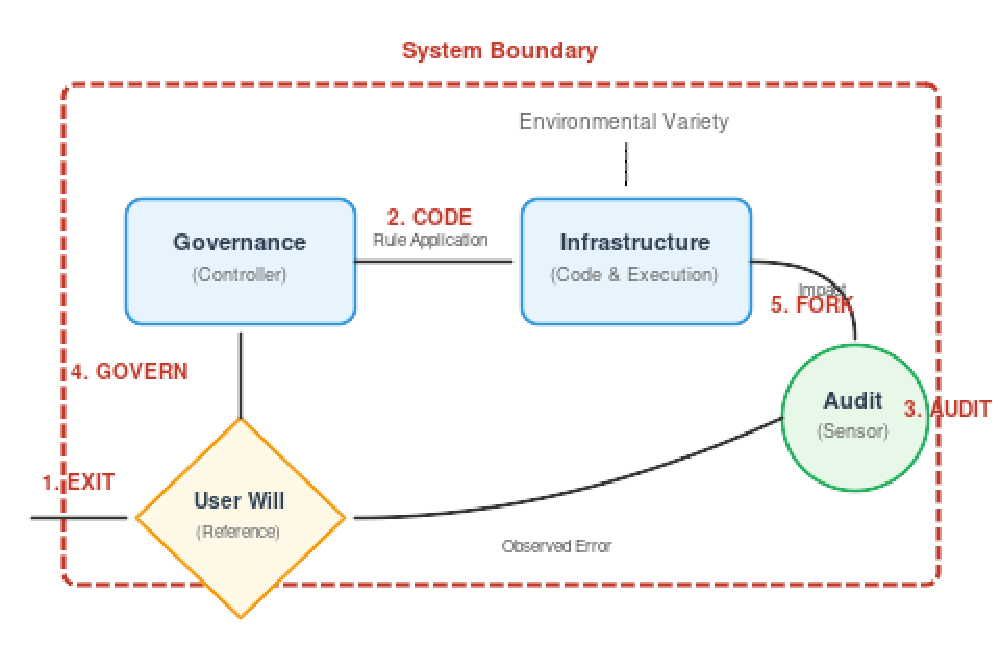
\includegraphics[width=0.75\textwidth]{figures/topology-of-necessity.pdf}
\caption{\textbf{Topology of Necessity.} Each corrigibility test corresponds to a breakage point in the feedback control loop.}
\label{fig:topology}
\end{figure}

\begin{figure}[H]
\centering
\begin{tikzpicture}[scale=0.85,
    tradition/.style={rectangle, rounded corners, draw=gray, fill=gray!10, minimum width=2.4cm, minimum height=0.7cm, font=\small},
    test/.style={rectangle, rounded corners, draw=#1, fill=#1!15, minimum width=1.5cm, minimum height=0.6cm, font=\small\bfseries},
    arrow/.style={-{Stealth[length=2mm]}, gray, thick}
]
% Three traditions at top
\node[tradition] (cyber) at (0,2.5) {Cybernetics};
\node[tradition] (commons) at (4,2.5) {Commons};
\node[tradition] (foss) at (8,2.5) {Free Software};

% Five tests at bottom
\node[test=exitcolor] (exit) at (0,0) {EXIT};
\node[test=codecolor] (code) at (2,0) {CODE};
\node[test=auditcolor] (audit) at (4,0) {AUDIT};
\node[test=governcolor] (govern) at (6,0) {GOVERN};
\node[test=forkcolor] (fork) at (8,0) {FORK};

% Connections - Cybernetics
\draw[arrow] (cyber.south) -- (exit.north);
\draw[arrow] (cyber.south) -- (audit.north west);

% Connections - Commons
\draw[arrow] (commons.south) -- (audit.north);
\draw[arrow] (commons.south) -- (govern.north);

% Connections - FOSS
\draw[arrow] (foss.south) -- (code.north east);
\draw[arrow] (foss.south) -- (fork.north);

% Labels
\node[font=\scriptsize, gray] at (4,-0.7) {All five tests required. Failure of any one disqualifies.};
\end{tikzpicture}
\caption{Five corrigibility tests derived from three independent theoretical traditions.}
\label{fig:framework}
\end{figure}

\subsection{Structural Symmetry of Power}

The five tests, while derived from distinct intellectual traditions, share a common organizing principle. Each enforces a constraint on power concentration at a different layer of the system. Together, they form a single power invariant:

\begin{center}
\begin{tabular}{@{}lll@{}}
\toprule
\textbf{Layer} & \textbf{Test} & \textbf{Function (Cybernetic)} \\
\midrule
Individual & EXIT & Reversibility of participation \\
Logic & CODE & Inspectability of rules \\
Logic & AUDIT & Verifiability of error \\
System & GOVERN & Constraint on controller variance \\
Ecosystem & FORK & Selection pressure via reproduction \\
\bottomrule
\end{tabular}
\end{center}

Each test enforces the same principle: \textit{No actor exercising power may be the sole judge of its continuation, scope, or correction.}

A system without EXIT is coercive. A system without GOVERN is arbitrary. A system without FORK is captive.

\subsection{Layer-Decomposed Evaluation}
\label{subsec:layers}

Complex infrastructure frequently stratifies into distinct functional layers, each with independent governance, transparency, and reproducibility properties. The five tests must be applied to each layer separately when:

\begin{enumerate}[noitemsep,topsep=0pt]
    \item Different entities control different layers (protocol versus implementation versus trust framework)
    \item Transparency varies across layers (open protocol, closed switching logic)
    \item Forkability differs by layer (code is forkable, network effects are not)
\end{enumerate}

\subsubsection{Propagation Rule}

A system that passes a test at one layer but fails at another does not achieve ``partial'' compliance. It fails the test. The evaluation proceeds from the layer closest to user impact upward; failure at any layer propagates to the whole.

Formally: Let $L_1, L_2, \ldots, L_n$ be the layers of a system, ordered by proximity to user impact. For test $T$:

\begin{equation}
T_{\text{system}} = \bigwedge_{i=1}^{n} T(L_i)
\end{equation}

The system passes $T$ if and only if every layer passes $T$.

\subsubsection{Application to Identity Infrastructure}

\begin{table}[htbp]
\centering
\small
\begin{tabular}{@{}llp{5cm}@{}}
\toprule
\textbf{Layer} & \textbf{Example Components} & \textbf{Typical Failure Mode} \\
\midrule
Protocol & W3C DID, VC Data Model & Often passes CODE \\
Implementation & Specific resolver, wallet software & May fail CODE (proprietary) \\
Credential & Issuer policies, attribute schemas & Often fails GOVERN (unilateral issuer) \\
Trust & Relying party acceptance, trusted lists & Often fails FORK (cannot reproduce acceptance) \\
\bottomrule
\end{tabular}
\caption{Identity infrastructure layer decomposition}
\label{tab:identity_layers}
\end{table}

The UPI payment rail exhibits similar layering: the protocol specification (NPCI-published) passes CODE at the protocol layer, but the switching logic (NPCI-operated) fails CODE at the implementation layer. Since the implementation layer is closer to user impact, the system fails CODE.

\subsubsection{The Weakest-Layer Principle}

This propagation rule has a counterintuitive but structurally necessary consequence: a system's corrigibility status equals its weakest layer across any test dimension. Strength at one layer cannot compensate for failure at another.

This principle prevents a common evasion: claiming corrigibility by publishing peripheral artifacts while retaining control over the layers that determine outcomes. Open-washing (Section~\ref{subsec:openwashing}) typically exploits layer confusion. Releasing SDKs (passing CODE at the interface layer) while keeping core logic proprietary (failing CODE at the execution layer) does not produce partial corrigibility. It produces total failure at the execution layer, which propagates to the system determination.

\section{The Dynamics of Incorrigibility}
\label{sec:dynamics}

The five tests define the static architecture of a corrigible system. However, infrastructure exists in time. When we apply these structural requirements to dynamic systems, three fundamental implications emerge regarding stability, energy conservation, and the rule of law. These principles explain why centralized grievance redressal mechanisms---the standard answer of bureaucracies to error---are mathematically insufficient to guarantee stability.

\subsection{The Correction Velocity Inequality}
\label{subsec:velocity}

Stability in a cybernetic system is not merely a function of whether a correction path \textit{exists}, but of its \textit{latency} relative to error generation. A correction mechanism that is theoretically available (e.g., a court case or a legislative amendment) but slower than the rate of divergence creates a runaway failure state.

We posit the \textbf{Temporal Stability Condition}: A system is corrigible only if the rate of effective correction ($C$) exceeds the rate of error accumulation ($E$) caused by environmental variety.

\begin{equation}
\frac{d}{dt} C(t) > \frac{d}{dt} E(t)
\end{equation}

$E(t)$ is driven by environmental volatility---identity fraud tactics, software exploits, pandemics, or economic shocks. These phenomena tend to grow exponentially or appear in high-velocity impulse shocks. In contrast, centralized governance operates on \textbf{bureaucratic time}. Legislative changes and judicial reviews are measured in months or years, while technical errors accumulate on \textbf{digital time}, measured in milliseconds. Appendix~\ref{appendix:proofs} provides a formal control-theoretic treatment of these claims; no additional assumptions beyond those stated here are introduced.

\begin{equation}
\frac{dC_{\text{bureaucratic}}}{dt} \ll \frac{dE_{\text{digital}}}{dt}
\end{equation}

This timescale mismatch is an instance of the Collingridge Dilemma \citep{collingridge1980}: a double-bind in technology governance. Early in a technology's development, change is easy but the need for change cannot be foreseen (the information problem). Later, when impacts become clear, change has become expensive, difficult, and time-consuming because the technology is entrenched (the power problem).

Digital Public Infrastructure exhibits the Collingridge Dilemma in acute form. By the time exclusion effects are documented (starvation deaths, banking denials, welfare failures), a system may have achieved mandatory status. Correction now requires not merely technical modification but legal amendment, bureaucratic reorganization, and political will. The system's success in achieving scale has made it resistant to correction.

Corrigibility is the structural response to this dilemma: build the correction mechanisms before the need for correction is apparent. EXIT, CODE, AUDIT, GOVERN, and FORK are not remedies applied after failure; they are architectural features that must be present from deployment. A system without these features will eventually require correction but will lack the capacity to receive it.

This inequality explains the failure of the ``post-execution'' remedies discussed in Section 4.4. Mechanisms like ombudsmen or grievance redressal officers inherently operate at a lower bandwidth and higher latency than the systems they supervise. When the correction loop is thermodynamically too slow to manage the entropy of the environment, error accumulates in the system until it suffers catastrophic collapse. Corrigibility requires closing the gap between error generation and correction; this is only possible if correction logic operates within the technical loop (Test 4), not outside it.

\subsection{The Conservation of Correction Demand}

When a system fails to correct errors due to the velocity mismatch described above, the demand for correction does not evaporate. It transforms. We propose a principle of \textbf{Conservation of Correction Demand}: for a given system state, the total pressure for correction is constant.

\begin{equation}
F_{\text{designed}} + F_{\text{emergent}} = K
\end{equation}

Here, $F_{\text{designed}}$ represents the flow of correction through designed channels---principally \textbf{EXIT} (reducing participation) and \textbf{GOVERN} (altering rules). When these channels are structurally blocked or throttled by bureaucracy, the pressure shifts to $F_{\text{emergent}}$. Emergent correction channels take the form of protest, litigation, hacks, grey markets, and eventually, civil unrest.

System operators can choose \textit{where} correction occurs; they cannot choose \textit{whether} it occurs. By suppressing EXIT (via mandatory laws) and blocking GOVERN (via executive fiat), authorities force correction demand into channels that are slower, costlier, and fundamentally more destabilizing to the social order. Corrigibility acts as a pressure relief valve that converts potential volatility into system evolution.

\subsubsection{Grievance Is Not Feedback}
\label{subsec:grievance}

A critical distinction must be drawn between \textit{grievance} and \textit{governance}. Many incorrigible systems act as ``roach motels'' for complaints: they allow users to submit unlimited feedback ($G$), but the system state ($S$) remains invariant to that input.

\begin{equation}
\frac{\partial S}{\partial G} = 0
\end{equation}

Grievance channels that record dissatisfaction without a binding mechanism to modify execution, policy, or eligibility logic do not constitute a feedback loop. They serve an aesthetic function, mimicking responsiveness while preserving the controller's rigidity. Under Ashby's Law, if the controller's response variety does not increase in response to signal, regulation has failed.

\subsection{The Structural Preconditions of Law}

These dynamics have profound implications for constitutional review. Legal doctrines such as proportionality analysis presuppose that state intrusions can be measured, minimized, and remedied. However, modern digital systems frequently violate the structural assumptions upon which these legal doctrines rest.

A court cannot apply proportionality review to a system whose execution is opaque (\textbf{CODE}). A legislature cannot remedy harm if the mechanism of harm is an irreversible digital transaction (\textbf{EXIT}). A regulator cannot oversee a system if they lack the technical capability to inspect it independent of the operator (\textbf{AUDIT}).

Where digital systems block these channels structurally, the rule of law becomes a legal fiction. External review mechanisms cannot function meaningfully if the internal architecture is designed to resist observation and modification. Therefore, \textbf{corrigibility} should be understood not merely as a technical specification, but as the \textit{evidentiary precondition} required for the law to take hold of the machine.

\section{Extension to Learned Systems}
\label{sec:learned}

The application of this framework to Artificial Intelligence requires resolving a fundamental crisis of verification. Earlier formulations of the five tests implicitly assumed a deterministic architecture, where the source code is the sole arbiter of behavior, inspection reveals logic, and exact reproduction is mechanically trivial. Learned systems (AI and ML models) dismantle these assumptions. In these systems, identical inputs may yield stochastic outputs; behavior is defined by training data rather than logic gates; and opacity is often an inherent property of the representation rather than a contrivance of the operator.

However, the collapse of deterministic transparency does not invalidate the structural necessity of corrigibility. To the contrary, as the system's internal logic becomes less intelligible to human operators, the external capacity for correction becomes more critical. \textbf{The five tests remain invariant; only the evidentiary standard changes.}

\subsection{The Invariance of the Standard}

\begin{proposition}
The five corrigibility tests remain invariant for learned systems. What changes is the verification method.
\end{proposition}

The table below illustrates how the mechanical verification of each test adapts to the probabilistic nature of AI without softening the structural requirement.

\begin{table}[htbp]
\centering
\begin{tabular}{@{}lll@{}}
\toprule
\textbf{Test} & \textbf{Deterministic Verification} & \textbf{Learned System Verification} \\
\midrule
EXIT & Can refuse the system & Disclosure + non-AI alternative \\
CODE & Source code determines behavior & Layered transparency across training pipeline \\
AUDIT & Inspect logic and outputs & Statistical bounds + continuous monitoring \\
GOVERN & Maintainer and RFC process & Governance over objectives and value tradeoffs \\
FORK & Copy code and deploy & Resource forkability (compute + data) \\
\bottomrule
\end{tabular}
\caption{Verification methods for deterministic vs. learned systems}
\end{table}

\subsection{What Is ``Source'' in a Learned System?}

A central challenge in complying with the \textbf{CODE} test is redefining the object of inspection. In a learned system, behavior is distributed across a lineage of distinct artifacts. The inference code is merely the execution engine; the actual behavioral logic is encoded in the weights, which are in turn downstream of the training corpus, filtering decisions, and RLHF preferences.

Therefore, publishing inference code alone does not satisfy the CODE test. It allows an auditor to run the machine, but not to understand why it produces specific outputs. To bridge this gap, compliance requires structured disclosure across the training pipeline, such as \textbf{Data Sheets for Datasets} \citep{gebru2021} and \textbf{Model Cards} \citep{mitchell2019}. These artifacts function as the ``source code'' for structural evaluation; withholding them renders the system a black box.

\subsection{The Temporal Variety Gap}

Unlike traditional software, which remains static until explicitly patched, learned systems possess a distinct vulnerability related to time. The variety of the controller ($V_c$) is frozen at the moment of training parameterization ($\theta$), while the variety of the world it operates upon ($V_d$) continues to expand.

\begin{equation}
\Delta(t) = V(\text{disturbance}; t) - V(\text{controller}; \theta)
\end{equation}

Without mechanisms for retraining or fine-tuning accessible to the community, the variety gap $\Delta(t)$ widens over time. Thus, AI corrigibility is not a deployment property, but a \textit{persistence condition}.

\begin{figure}[htbp]
\centering
\begin{tikzpicture}[x=0.8cm, y=0.5cm, font=\sffamily]

    % Axes
    \draw[->, thick, gray] (0,0) -- (10,0) node[right] {Time ($t$)};
    \draw[->, thick, gray] (0,0) -- (0,8) node[above] {Variety ($V$)};

    % Real World Complexity (The Disturbance) - Curving up
    \draw[thick, forkcolor, smooth] plot coordinates {(0,1) (2,1.8) (4,3.5) (6,4.5) (8,7.5) (9.5, 9)};
    \node[forkcolor, anchor=west, font=\scriptsize] at (9.5, 9) {$V(\text{Environment})$};

    % AI Model State (The Controller) - Step Function
    \draw[thick, codecolor] (0,1) -- (4,1);
    \draw[dashed, gray] (4,1) -- (4,3.5);
    \draw[thick, codecolor] (4,3.5) -- (8,3.5);
    \draw[dashed, gray] (8,3.5) -- (8,7.5);
    \draw[thick, codecolor] (8,7.5) -- (9.5,7.5);

    % Labels for Model
    \node[codecolor, anchor=north, font=\scriptsize] at (2,1) {Model $\theta_1$};
    \node[codecolor, anchor=north, font=\scriptsize] at (6,3.5) {Model $\theta_2$};

    % The Gap (Error)
    \fill[red!10] (0,1) -- (4,1) -- (4,3.5) -- plot[smooth] coordinates {(4,3.5) (2,1.8) (0,1)} -- cycle;
    \fill[red!20] (4,3.5) -- (8,3.5) -- (8,7.5) -- plot[smooth] coordinates {(8,7.5) (6,4.5) (4,3.5)} -- cycle;

    % Annotations
    \node[anchor=west, text=red!80!black, font=\scriptsize] at (0.5, 2.5) {$\Delta(t)$};
    \draw[->, red!80!black] (1.2, 2.3) -- (1.5, 1.5);

    \node[align=center, font=\tiny, gray] at (4, -1) {\textbf{Retraining}\\(FORK)};
    \draw[->, gray, dotted] (4, -0.3) -- (4, 0.8);

\end{tikzpicture}
\caption{\textbf{The Temporal Variety Gap.} Environmental variety $V(e)$ evolves continuously (curve). A fixed model $\theta$ (stepped line) diverges from reality. The shaded area represents accumulated error. Only \textbf{FORK} rights allow the gap to be closed via retraining.}
\label{fig:variety_gap}
\end{figure}

\subsection{Resource Barriers to Forkability}

The right to \textbf{FORK} a learned system is constrained by physical resources rather than just copyright. In traditional software, the cost to fork is the cost of storage; in AI, the cost to fork is the cost of compute.

\begin{table}[htbp]
\centering
\begin{tabular}{@{}lll@{}}
\toprule
\textbf{Layer} & \textbf{Cost} & \textbf{Barrier} \\
\midrule
Inference code & Minimal & None \\
Running open weights & Low & Minor \\
Fine-tuning & Moderate & Economic \\
Retraining from scratch & Very high & Structural \\
\bottomrule
\end{tabular}
\caption{Resource barriers to forking learned systems}
\end{table}

If a community has the legal right to fork a model but lacks access to the original training data or the massive compute clusters required to reproduce it, the ``Fork'' is illusory.

\begin{claim}
Legal permission to fork without access to compute or data is meaningless. This is an infrastructure question, not a licensing question.
\end{claim}

\section{Empirical Evaluation}
\label{sec:diagnosis}

To demonstrate the framework's application, we evaluate systems across three categories: government infrastructure promoted as ``DPI,'' platform infrastructure claiming ``openness,'' and infrastructure that satisfies all five tests.

\subsection{Government Infrastructure: The Trap of Partial Compliance}

Government-operated systems currently designated as Digital Public Infrastructure frequently exhibit a dangerous failure mode: they achieve partial compliance on technical tests (EXIT, CODE, AUDIT) while failing structurally on governance tests (GOVERN, FORK). By capturing the monopoly on execution, they render the feedback loop inoperable.

\begin{table}[htbp]
    \centering
    \caption{\textbf{Evaluation of Government Infrastructure.} Centralized execution leads to consistent structural failure despite ``open standards'' rhetoric.}
    \label{tab:govt_infra}

    % --- Subtable A: Aadhaar ---
    \begin{subtable}{1\textwidth}
        \centering
        \caption{Aadhaar (India) -- Mandatory ID}
        \small
        \begin{tabular}{@{}llp{8.5cm}@{}}
            \toprule
            \textbf{Test} & \textbf{Result} & \textbf{Evidence} \\
            \midrule
            EXIT & \textcolor{red}{FAIL} & Disproportionate penalty: exclusion from PDS, banking, SIM \citep{khera2019}. \\
            CODE & \textcolor{red}{FAIL} & Execution logic opaque: proprietary matcher, closed algorithms. \\
            AUDIT & \textcolor{red}{FAIL} & External testing prohibited: independent error measurement illegal. \\
            GOVERN & \textcolor{red}{FAIL} & No binding constraint: UIDAI is both operator and regulator. \\
            FORK & \textcolor{red}{FAIL} & No legal/technical/economic means: total centralized capture. \\
            \bottomrule
        \end{tabular}
        \vspace{0.3cm}
    \end{subtable}

    % --- Subtable B: UPI ---
    \begin{subtable}{1\textwidth}
        \centering
        \caption{UPI (India) -- Payment Rail}
        \small
        \begin{tabular}{@{}llp{8.5cm}@{}}
            \toprule
            EXIT & \textcolor{orange}{PARTIAL} & Reduced penalty: cash exists but network effects coerce. \\
            CODE & \textcolor{orange}{PARTIAL} & Partial inspection: protocol specs open, switching logic closed. \\
            AUDIT & \textcolor{orange}{PARTIAL} & Limited testing: regulator audits, public measurement blocked. \\
            GOVERN & \textcolor{red}{FAIL} & No binding constraint: banks own NPCI, regulate themselves. \\
            FORK & \textcolor{red}{FAIL} & No economic means: hub-and-spoke requires NPCI cooperation. \\
            \bottomrule
        \end{tabular}
        \vspace{0.3cm}
    \end{subtable}

    % --- Subtable C: Pix ---
    \begin{subtable}{1\textwidth}
        \centering
        \caption{Pix (Brazil) -- Central Bank Payment}
        \small
        \begin{tabular}{@{}llp{8.5cm}@{}}
            \toprule
            \textbf{Test} & \textbf{Result} & \textbf{Evidence} \\
            \midrule
            EXIT & \textcolor{orange}{PARTIAL} & Reduced penalty: cash and cards exist; digital-only services coerce adoption. \\
            CODE & \textcolor{orange}{PARTIAL} & Partial inspection: API specification public; central routing logic closed. \\
            AUDIT & \textcolor{orange}{PARTIAL} & Limited testing: aggregate statistics public; independent error measurement blocked. \\
            GOVERN & \textcolor{red}{FAIL} & No binding constraint: BCB sets and enforces Pix rules unilaterally. \\
            FORK & \textcolor{red}{FAIL} & No reproduction means: central switch requires BCB; no independent implementation. \\
            \bottomrule
        \end{tabular}
        \vspace{0.3cm}
    \end{subtable}

    % --- Subtable D: X-Road ---
    \begin{subtable}{1\textwidth}
        \centering
        \caption{X-Road (Estonia/Nordic) -- Data Exchange Layer}
        \small
        \begin{tabular}{@{}llp{8.5cm}@{}}
            \toprule
            \textbf{Test} & \textbf{Result} & \textbf{Evidence} \\
            \midrule
            EXIT & \textcolor{red}{FAIL} & Disproportionate penalty: exclusion from government services. \\
            CODE & \textcolor{green!50!black}{PASS} & Execution logic inspectable: MIT source on GitHub. \\
            AUDIT & \textcolor{green!50!black}{PASS} & External testing possible: transaction logs, documented APIs. \\
            GOVERN & \textcolor{green!50!black}{PASS} & Binding constraint: NIIS treaty, MIT license irrevocable. \\
            FORK & \textcolor{green!50!black}{PASS} & Legal + technical + economic: 25+ country deployments prove feasibility. \\
            \bottomrule
        \end{tabular}
        \vspace{0.3cm}
    \end{subtable}

    % --- Subtable E: UK Open Banking ---
    \begin{subtable}{1\textwidth}
        \centering
        \caption{UK Open Banking -- Regulated API Standard}
        \small
        \begin{tabular}{@{}llp{8.5cm}@{}}
            \toprule
            EXIT & \textcolor{orange}{PARTIAL} & Can revoke API consent; cannot exit banking system. \\
            CODE & \textcolor{red}{FAIL} & Execution logic not inspectable: bank implementations proprietary. \\
            AUDIT & \textcolor{green!50!black}{PASS} & External testing: FCA oversight, TPP certification. \\
            GOVERN & \textcolor{green!50!black}{PASS} & Binding constraint: CMA order, PSD2 regulation. \\
            FORK & \textcolor{orange}{PARTIAL} & Legal rights exist; economic means require regulatory recognition. \\
            \bottomrule
        \end{tabular}
    \end{subtable}
\end{table}

\textbf{Pattern}: X-Road (4/5) fails only EXIT. UK Open Banking (2/5) passes AUDIT and GOVERN but fails CODE: the API \textit{specification} is public, but the bank \textit{implementations} are proprietary. Specification $\neq$ Code. You can see the interface; you cannot inspect the execution.

\subsection{Platform Infrastructure: The Illusion of Openness}

In the private sector, systems often leverage "open source" branding while retaining centralized control. This decoupling of artifact transparency from governance reality creates a distinct failure pattern: the artifacts are public; the decisions are not.

\begin{table}[htbp]
    \centering
    \caption{\textbf{Evaluation of Private/Platform Infrastructure.} Technical openness (Source/Weights) does not guarantee structural accountability.}
    \label{tab:corp_infra}

    % --- Subtable A: Open Weights AI ---
    \begin{subtable}{1\textwidth}
        \centering
        \caption{Open-Weights AI (Llama, etc.)}
        \small
        \begin{tabular}{@{}llp{8.5cm}@{}}
            \toprule
            \textbf{Test} & \textbf{Result} & \textbf{Evidence} \\
            \midrule
            EXIT & \textcolor{green!50!black}{PASS} & No disproportionate penalty: can run locally, switch models freely. \\
            CODE & \textcolor{orange}{PARTIAL} & Partial inspection: weights public; training data and RLHF opaque. \\
            AUDIT & \textcolor{orange}{PARTIAL} & Limited testing: black-box probing possible; lineage unverifiable. \\
            GOVERN & \textcolor{red}{FAIL} & No binding constraint: firm sets safety/capability trade-offs unilaterally. \\
            FORK & \textcolor{orange}{PARTIAL} & Partial means: fine-tuning possible; retraining blocked by compute cost. \\
            \bottomrule
        \end{tabular}
        \vspace{0.3cm}
    \end{subtable}

    % --- Subtable B: Android ---
    \begin{subtable}{1\textwidth}
        \centering
        \caption{Android (AOSP + GMS)}
        \small
        \begin{tabular}{@{}llp{8.5cm}@{}}
            \toprule
            \textbf{Test} & \textbf{Result} & \textbf{Evidence} \\
            \midrule
            EXIT & \textcolor{orange}{PARTIAL} & Moderate penalty: device portable; ecosystem lock-in creates friction. \\
            CODE & \textcolor{orange}{PARTIAL} & Partial inspection: AOSP open; Play Services and Identity closed. \\
            AUDIT & \textcolor{orange}{PARTIAL} & Limited testing: OS auditable; Google Services behavior opaque. \\
            GOVERN & \textcolor{red}{FAIL} & No binding constraint: Google sets roadmap and certification unilaterally. \\
            FORK & \textcolor{orange}{PARTIAL} & Partial means: LineageOS exists; app ecosystem requires GMS. \\
            \bottomrule
        \end{tabular}
        \vspace{0.3cm}
    \end{subtable}

    % --- Subtable C: Signal ---
    \begin{subtable}{1\textwidth}
        \centering
        \caption{Signal Protocol}
        \small
        \begin{tabular}{@{}llp{8.5cm}@{}}
            \toprule
            \textbf{Test} & \textbf{Result} & \textbf{Evidence} \\
            \midrule
            EXIT & \textcolor{green!50!black}{PASS} & No disproportionate penalty: can switch to alternatives freely. \\
            CODE & \textcolor{green!50!black}{PASS} & Full inspection: client and server source available (GPL/AGPL). \\
            AUDIT & \textcolor{green!50!black}{PASS} & External testing: cryptographic properties independently verifiable. \\
            GOVERN & \textcolor{red}{FAIL} & No binding constraint: Foundation board sets direction unilaterally. \\
            FORK & \textcolor{red}{FAIL} & No economic means: code forkable but no federation locks network effects. \\
            \bottomrule
        \end{tabular}
    \end{subtable}
\end{table}

\textbf{Pattern: Asymmetric Openness.} These systems deploy strategic openness: releasing artifacts for ecosystem capture while retaining governance. This satisfies CODE (inspection possible) while failing GOVERN (correction blocked). The framework distinguishes artifact transparency (can you see the code?) from governance accountability (can you correct the system?). Open weights, open protocols, and open standards can each mask closed correction loops. ``Open weights'' $\neq$ ``open.'' ``Open source'' $\neq$ ``accountable.'' The artifact is open. The correction loop is closed. Seeing the machine does not govern it.

\subsection{Corrigible Infrastructure}

For contrast, Table~\ref{tab:positive} summarizes seventeen systems that pass all five tests. A striking pattern emerges: these systems are predominantly non-essential infrastructure. No individual's survival depends on accessing Linux or Let's Encrypt. This correlation between corrigibility and non-essentiality is not coincidental; it reflects the structural tension analyzed in Section~\ref{subsec:essential}.

\begin{table}[htbp]
\centering
\small
\renewcommand{\arraystretch}{1.3}
\begin{tabular}{@{}l>{\raggedright}p{3.2cm}>{\centering\arraybackslash}p{1.2cm}p{5.8cm}@{}}
\toprule
\rowcolor{gray!15}
\textbf{System} & \textbf{Steward} & \textbf{Score} & \textbf{Why Corrigible} \\
\midrule
\rowcolor{green!8}
Linux Kernel & Linux Foundation & \cellcolor{green!25}\textbf{5/5} & Fully reproducible. Full triad (legal, technical, economic) exists. Independent distributions prove forkability. \\
Let's Encrypt & ISRG & \cellcolor{green!25}\textbf{5/5} & Open source CA, IETF standards, nonprofit 501(c)(3) \\
\rowcolor{green!8}
Wikipedia & Wikimedia Foundation & \cellcolor{green!25}\textbf{5/5} & CC BY-SA content, public edit history, community RfC governance \\
Matrix Protocol & Matrix.org Foundation & \cellcolor{green!25}\textbf{5/5} & Apache 2.0, federated by design, self-hostable \\
\rowcolor{green!8}
Bluesky (AT Protocol) & Bluesky PBC & \cellcolor{green!25}\textbf{5/5} & MIT/Apache, portable DID identity, self-hostable PDS \\
PostgreSQL & PGDG & \cellcolor{green!25}\textbf{5/5} & BSD-like license, public mailing lists, major forks exist \\
\rowcolor{green!8}
IPFS & Protocol Labs & \cellcolor{green!25}\textbf{5/5} & MIT/Apache, public IPIP process, no token governance \\
Bitcoin & Decentralized & \cellcolor{green!25}\textbf{5/5} & MIT source, public BIP process, proven forks (BCH, BSV) \\
\rowcolor{green!8}
Kubernetes & CNCF & \cellcolor{green!25}\textbf{5/5} & Apache 2.0, KEP process, distributions (OpenShift, k3s) \\
Firefox & Mozilla Foundation & \cellcolor{green!25}\textbf{5/5} & MPL 2.0, nonprofit manifesto, forks (LibreWolf, Tor Browser) \\
\rowcolor{green!8}
Apache HTTP & Apache Foundation & \cellcolor{green!25}\textbf{5/5} & Apache 2.0 license, ASF governance, powers 30\% of web \\
Apache Kafka & Apache Foundation & \cellcolor{green!25}\textbf{5/5} & Apache 2.0, KIP process public, Fortune 500 standard \\
\rowcolor{green!8}
OpenSearch & Linux Foundation & \cellcolor{green!25}\textbf{5/5} & Forked from Elasticsearch; Apache 2.0, multi-vendor governance \\
Valkey & Linux Foundation & \cellcolor{green!25}\textbf{5/5} & Forked from Redis; BSD license, community governance restored \\
\rowcolor{green!8}
Hyperledger & LF Decentralized Trust & \cellcolor{green!25}\textbf{5/5} & Apache 2.0 framework; institutional deployments require separate evaluation \\
LibreOffice & Document Foundation & \cellcolor{green!25}\textbf{5/5} & Forked from OpenOffice; LGPL/MPL, nonprofit governance \\
\rowcolor{green!8}
MariaDB & MariaDB Foundation & \cellcolor{green!25}\textbf{5/5} & Forked from MySQL; GPL, foundation governance \\
Eclipse IDE & Eclipse Foundation & \cellcolor{green!25}\textbf{5/5} & EPL 2.0, 386 member orgs, committer-led governance \\
\bottomrule
\end{tabular}
\caption{Infrastructure systems satisfying all five corrigibility tests. All systems demonstrate full EXIT, CODE, AUDIT, GOVERN, and FORK compliance.}
\label{tab:positive}
\end{table}

\textbf{Fork as Correction}: OpenSearch, Valkey, LibreOffice, and MariaDB demonstrate Ashby's Law in practice. Each emerged when governance variety collapsed: Oracle's Sun acquisition (2010) triggered LibreOffice and MariaDB; unilateral license changes triggered OpenSearch (2021) and Valkey (2024). The ecosystem restored requisite variety through forking.

The framework is governance-agnostic: corporate participation is not disqualifying. Kubernetes (CNCF), Hyperledger, and Let's Encrypt all have significant corporate involvement while passing all tests. The test is whether governance permits correction, not who participates.

\textbf{License vs. Governance}: Redis Ltd. added AGPLv3 in 2025, restoring open licensing. But license is orthogonal to governance. \textit{License} determines what you may do with code; \textit{governance} determines who decides what it becomes. Redis passes one; Valkey passes both.

\subsection{The Taxonomy of Open-Washing}
\label{subsec:openwashing}

Systems that fail these structural tests frequently employ vocabulary to obscure their closure:
\begin{enumerate}
    \item \textbf{Standard-Washing}: Adopting open technical standards (like ISO/W3C) as proxy for governance accountability.
    \item \textbf{Open-Washing}: Releasing peripheral SDKs while keeping core execution logic proprietary.
    \item \textbf{Multilateral-Washing}: Using international endorsements (G20, WB) to substitute for technical auditability.
    \item \textbf{Safety-Washing}: Justifying opacity by claiming inspection poses a security risk.
    \item \textbf{Consent-Washing}: Obtaining formal consent under conditions of economic coercion.
    \item \textbf{DID-Washing}: Deploying decentralized identifiers without decentralized governance (see Section~\ref{subsubsec:didwashing}).
\end{enumerate}

\subsubsection{DID-Washing: The Layer Confusion Problem}
\label{subsubsec:didwashing}

Decentralized Identifiers (DIDs) present a distinct challenge to corrigibility evaluation because they separate technical decentralization from governance decentralization across multiple architectural layers. The W3C DID Core 1.0 specification \citep{w3cdid2022} defines DIDs as ``globally unique identifiers'' that ``do not require a centralized registration authority.'' This technical claim is accurate. However, a system can implement DIDs at the identifier layer while retaining centralized control at every layer that determines actual utility.

Identity infrastructure comprises at least four functional layers, each with independent governance:

\begin{table}[htbp]
\centering
\small
\begin{tabular}{@{}llp{5cm}@{}}
\toprule
\textbf{Layer} & \textbf{Function} & \textbf{DID-Washing Failure Mode} \\
\midrule
Identifier & Generate and resolve DIDs & Often decentralized, but meaningless alone \\
Credential & Issue verifiable claims about the subject & Usually centralized: single issuer dominates \\
Trust & Determine which credentials are accepted & Controlled by policy, trusted lists, or law \\
Revocation & Invalidate credentials or identifiers & Often requires issuer cooperation \\
\bottomrule
\end{tabular}
\caption{DID-washing failure modes by layer}
\label{tab:didwashing}
\end{table}

A DID that resolves correctly but is not accepted by any relying party is functionally equivalent to no identity at all. The identifier is ``self-sovereign''; the identity utility is not.

\paragraph{Empirical Examples.} The EU Digital Identity Wallet (EUDI) under eIDAS 2.0 \citep{eidas2024} illustrates sophisticated DID-washing. The architecture employs selective disclosure credentials and cryptographic proofs superficially similar to DID/VC ecosystems. However:

\begin{itemize}[noitemsep,topsep=0pt]
    \item Credential issuance for Person Identification Data is an exclusive government function.
    \item Trust determination requires registration in Member State Trusted Lists.
    \item Wallet certification depends on government-approved Qualified Trust Service Providers (QTSPs).
    \item Trusted Execution Environment dependency hands cryptographic key governance to mobile OS vendors (Google, Apple).
\end{itemize}

The result: users control their container (the wallet) but not their capability (the credentials). A journalist critical of their government holds a ``decentralized'' identifier that can be rendered useless by a single administrative act: revocation from the trusted list.

\paragraph{Consent-Washing: The DigiLocker Case.} India's DigiLocker exhibits a simpler failure mode. It does not claim to use DIDs; it uses centralized URIs and mandatory Aadhaar linkage. However, promotional language around ``user consent'' and ``digital empowerment'' obscures the structural reality: users cannot register without Aadhaar, cannot store documents outside government-controlled infrastructure, and cannot port their identity to alternative systems. This is not DID-washing but \textit{consent-washing}: the vocabulary of user control applied to a system that offers none.

\paragraph{Implications for Framework Application.} DID-washing exploits a gap in naive corrigibility evaluation. A system may appear to pass CODE (the DID spec is public) and FORK (anyone can implement the spec) while failing at the trust layer where actual power resides.

The framework must be applied layer by layer (see Section~\ref{subsec:layers}). For identity systems:

\begin{itemize}[noitemsep,topsep=0pt]
    \item CODE must be evaluated at each layer: identifier resolution, credential issuance logic, trust framework rules, and revocation mechanisms.
    \item GOVERN must ask: who controls the acceptance policy? If a single authority determines which credentials are valid, governance is centralized regardless of identifier architecture.
    \item FORK must ask: can a community reproduce the trust framework, not merely the identifier scheme? If relying parties are legally required to accept only government-issued credentials, forkability is illusory.
\end{itemize}

A system passes the DID-washing test only if decentralization extends through the full trust stack: issuance, verification, acceptance policy, and revocation governance. Technical decentralization at the identifier layer with governance centralization at the trust layer is structural theater.

\begin{claim}
Identifier decentralization is not system decentralization. The corrigibility of an identity system is determined by its weakest layer across any test dimension.
\end{claim}

\begin{figure}[htbp]
\centering
\begin{tikzpicture}[
    scale=0.85,
    pass/.style={fill=green!30},
    fail/.style={fill=red!30},
    partial/.style={fill=orange!30},
    header/.style={font=\scriptsize\bfseries},
    cell/.style={font=\scriptsize, minimum width=0.9cm, minimum height=0.5cm}
]
% Headers
\node[header] at (0,0) {};
\node[header, text=exitcolor] at (1.2,0) {EXIT};
\node[header, text=codecolor] at (2.2,0) {CODE};
\node[header, text=auditcolor] at (3.2,0) {AUDIT};
\node[header, text=governcolor] at (4.2,0) {GOV};
\node[header, text=forkcolor] at (5.2,0) {FORK};
\node[header] at (6.4,0) {Result};

% Aadhaar
\node[cell, anchor=east] at (-0.2,-0.6) {Aadhaar};
\node[cell, fail] at (1.2,-0.6) {\texttimes};
\node[cell, fail] at (2.2,-0.6) {\texttimes};
\node[cell, fail] at (3.2,-0.6) {\texttimes};
\node[cell, fail] at (4.2,-0.6) {\texttimes};
\node[cell, fail] at (5.2,-0.6) {\texttimes};
\node[cell, font=\scriptsize\bfseries, text=red] at (6.4,-0.6) {0/5};

% UPI
\node[cell, anchor=east] at (-0.2,-1.2) {UPI};
\node[cell, partial] at (1.2,-1.2) {\textasciitilde};
\node[cell, partial] at (2.2,-1.2) {\textasciitilde};
\node[cell, partial] at (3.2,-1.2) {\textasciitilde};
\node[cell, fail] at (4.2,-1.2) {\texttimes};
\node[cell, fail] at (5.2,-1.2) {\texttimes};
\node[cell, font=\scriptsize\bfseries, text=red] at (6.4,-1.2) {0/5};

% Pix
\node[cell, anchor=east] at (-0.2,-1.8) {Pix};
\node[cell, partial] at (1.2,-1.8) {\textasciitilde};
\node[cell, partial] at (2.2,-1.8) {\textasciitilde};
\node[cell, partial] at (3.2,-1.8) {\textasciitilde};
\node[cell, fail] at (4.2,-1.8) {\texttimes};
\node[cell, fail] at (5.2,-1.8) {\texttimes};
\node[cell, font=\scriptsize\bfseries, text=red] at (6.4,-1.8) {0/5};

% Open-weights AI
\node[cell, anchor=east] at (-0.2,-2.4) {Llama etc.};
\node[cell, pass] at (1.2,-2.4) {\checkmark};
\node[cell, partial] at (2.2,-2.4) {\textasciitilde};
\node[cell, partial] at (3.2,-2.4) {\textasciitilde};
\node[cell, fail] at (4.2,-2.4) {\texttimes};
\node[cell, partial] at (5.2,-2.4) {\textasciitilde};
\node[cell, font=\scriptsize\bfseries, text=red] at (6.4,-2.4) {1/5};

% Separator line
\draw[gray, thick] (-0.8,-2.9) -- (7,-2.9);

% Linux
\node[cell, anchor=east] at (-0.2,-3.4) {Linux};
\node[cell, pass] at (1.2,-3.4) {\checkmark};
\node[cell, pass] at (2.2,-3.4) {\checkmark};
\node[cell, pass] at (3.2,-3.4) {\checkmark};
\node[cell, pass] at (4.2,-3.4) {\checkmark};
\node[cell, pass] at (5.2,-3.4) {\checkmark};
\node[cell, font=\scriptsize\bfseries, text=green!50!black] at (6.4,-3.4) {5/5};

% Let's Encrypt
\node[cell, anchor=east] at (-0.2,-4.0) {Let's Enc.};
\node[cell, pass] at (1.2,-4.0) {\checkmark};
\node[cell, pass] at (2.2,-4.0) {\checkmark};
\node[cell, pass] at (3.2,-4.0) {\checkmark};
\node[cell, pass] at (4.2,-4.0) {\checkmark};
\node[cell, pass] at (5.2,-4.0) {\checkmark};
\node[cell, font=\scriptsize\bfseries, text=green!50!black] at (6.4,-4.0) {5/5};

% Kubernetes (CNCF)
\node[cell, anchor=east] at (-0.2,-4.6) {K8s};
\node[cell, pass] at (1.2,-4.6) {\checkmark};
\node[cell, pass] at (2.2,-4.6) {\checkmark};
\node[cell, pass] at (3.2,-4.6) {\checkmark};
\node[cell, pass] at (4.2,-4.6) {\checkmark};
\node[cell, pass] at (5.2,-4.6) {\checkmark};
\node[cell, font=\scriptsize\bfseries, text=green!50!black] at (6.4,-4.6) {5/5};

% Bitcoin (Decentralized)
\node[cell, anchor=east] at (-0.2,-5.2) {Bitcoin};
\node[cell, pass] at (1.2,-5.2) {\checkmark};
\node[cell, pass] at (2.2,-5.2) {\checkmark};
\node[cell, pass] at (3.2,-5.2) {\checkmark};
\node[cell, pass] at (4.2,-5.2) {\checkmark};
\node[cell, pass] at (5.2,-5.2) {\checkmark};
\node[cell, font=\scriptsize\bfseries, text=green!50!black] at (6.4,-5.2) {5/5};

% +15 more (reference)
\node[cell, anchor=east, font=\scriptsize\itshape, text=gray] at (-0.2,-5.8) {+15 more};
\node[cell, font=\scriptsize, text=gray] at (3.2,-5.8) {See Table~\ref{tab:positive}};

% Legend
\node[font=\tiny, gray] at (3.2,-6.4) {\checkmark = Pass \quad \textasciitilde\ = Partial \quad \texttimes\ = Fail};
\end{tikzpicture}
\caption{Comparative evaluation summary. Systems labeled ``DPI'' (above line) fail structural tests. Corrigible infrastructure (below line) passes all five. See Table~\ref{tab:positive} for complete list.}
\label{fig:comparison}
\end{figure}

\subsection{Implications}

The contrast is instructive. Aadhaar and UPI, promoted as model DPI, fail all tests. The seventeen systems in Table~\ref{tab:positive}, rarely described as ``DPI,'' pass all tests.

This suggests the ``public'' in Digital Public Infrastructure often refers to \textit{population-scale deployment} rather than \textit{public accountability}. The framework distinguishes these: scale is not governance.

All systems that pass share common properties:
\begin{itemize}
    \item Open source with permissive or copyleft licensing
    \item Nonprofit or community governance structures
    \item Protocol standardization through open processes (IETF, LKML)
    \item No monopoly on essential services
\end{itemize}

Scale does not require capture. Universality does not require opacity. The choice is architectural.

\section{Discussion}
\label{sec:discussion}

\subsection{The Cybernetics of Binary Evaluation}

Critics often argue that this framework's binary pass/fail topology is too rigid for the complex reality of governance, proposing instead "maturity models" or graded scorecards. From a cybernetic perspective, we reject this gradation. Corrigibility is not a variable virtue; it is a \textbf{structural connectivity state}.

In a control system, a feedback loop is either closed or it is open. There is no such thing as a "mostly closed" loop. A wire that is disconnected by 1 millimeter transmits zero signal.

\begin{itemize}
    \item A system that allows \textbf{AUDIT} (Sensing) but blocks \textbf{GOVERN} (Actuation) is an \textbf{Open Loop}. It observes errors but cannot fix them.
    \item A system that allows \textbf{GOVERN} but blocks \textbf{EXIT} is a \textbf{Coercive Loop}. It traps energy inside the system until it fails catastrophically.
\end{itemize}

Partial compliance creates "zombie infrastructure"---systems that maintain the aesthetic of responsiveness while severing the actual capacity for stability. Therefore, a "Partial" score in this framework represents a \textbf{Fatal Structural Failure}. A system is either corrigible, or it is not.

The binary model is a deliberate analytical choice. Real systems exhibit continuous variation in feedback quality: channels may be partially blocked, signals degraded but not absent, corrections slow but not entirely unavailable. The binary classification discards this nuance for structural clarity.

This trade-off is justified on two grounds. First, the regulatory purpose: a system either meets the threshold for public legitimacy or it does not. Graduated compliance creates negotiation space that operators exploit. Second, the cybernetic purpose: a feedback loop either closes or it does not. Partial closure is a category error; a wire that transmits 50\% of the signal does not produce 50\% of the regulation.

For diagnostic purposes, gradation remains useful. The auditor schema (Appendix~\ref{appendix:schema}) preserves continuous measurements in fields like \texttt{penalty\_ratio}, \texttt{visibility}, and \texttt{fix\_latency\_observed}. The binary determination is the output; the continuous measurements are the inputs. Evaluators can examine the inputs to prioritize interventions even when the output is uniformly ``fail.''

\begin{figure}[htbp]
\centering
\begin{tikzpicture}[
    scale=0.85, transform shape,
    box/.style={rectangle, draw=gray!60, thick, fill=white, rounded corners, minimum height=0.8cm, minimum width=1.5cm, font=\scriptsize\sffamily},
    lbl/.style={font=\tiny\sffamily\bfseries, color=gray},
    cross/.style={path picture={
        \draw[red, thick] (path picture bounding box.south west) -- (path picture bounding box.north east);
        \draw[red, thick] (path picture bounding box.south east) -- (path picture bounding box.north west);
    }}
]

% --- ROW 1: CORRIGIBLE (Closed Loop) ---
\node[font=\bfseries\sffamily, align=left] at (-3, 0) {1. CORRIGIBLE\\(Closed Loop)};
\node[box, fill=green!5] (op1) at (0,0) {Operator};
\node[box, fill=green!5] (us1) at (4,0) {Public};

\draw[->, thick, codecolor] (op1) -- node[above, font=\tiny] {Action} (us1);
\draw[->, thick, exitcolor] (us1) -- node[below, font=\tiny] {EXIT/Correction} (op1);

\node[right=0.5cm of us1, font=\tiny\sffamily, text width=2cm, align=left, color=green!40!black] {
    \textbf{Stable}\\
    Error signals reduce variance.
};

% --- ROW 2: COERCIVE (No Exit) ---
\node[font=\bfseries\sffamily, align=left] at (-3, -2) {2. COERCIVE\\(No Exit)};
\node[box] (op2) at (0,-2) {Operator};
\node[box, fill=red!5] (us2) at (4,-2) {Public};

\draw[->, thick, codecolor] (op2) -- node[above, font=\tiny] {Mandate} (us2);
\draw[->, thick, exitcolor, dashed] (us2.south) -- +(0,-0.4) -| (op2.south);
\node[circle, fill=white, draw=red, inner sep=1pt, cross] at (2, -2.6) {};
\node[below, font=\tiny, color=red] at (2, -2.7) {Blocked (Aadhaar)};

\node[right=0.5cm of us2, font=\tiny\sffamily, text width=2cm, align=left, color=red!40!black] {
    \textbf{Unstable}\\
    Variance accumulates until rupture.
};

% --- ROW 3: OPAQUE (No Inspection) ---
\node[font=\bfseries\sffamily, align=left] at (-3, -4) {3. OPAQUE\\(No Insight)};
\node[box, fill=gray!20] (op3) at (0,-4) {AI Model};
\node[box] (us3) at (4,-4) {Public};

\draw[->, thick, codecolor, dashed] (op3) -- node[above, font=\tiny] {????} (us3);
\node[circle, fill=white, draw=auditcolor, inner sep=1pt, cross] at (2, -4) {};
\node[below, font=\tiny, color=auditcolor] at (2, -4.1) {Hidden Logic (Black Box)};

\draw[->, thick, exitcolor] (us3.south) -- +(0,-0.4) -| (op3.south);

\node[right=0.5cm of us3, font=\tiny\sffamily, text width=2cm, align=left, color=orange!40!black] {
    \textbf{Drifting}\\
    Feedback irrelevant (signal noise).
};

\end{tikzpicture}
\caption{\textbf{Topologies of Failure.}
(1) A corrigible system closes the loop, converting error signals into stability.
(2) A coercive system blocks \textbf{EXIT}, trapping energy.
(3) An opaque system obscures the action channel, making feedback unintelligible.}
\label{fig:failure_modes}
\end{figure}

\subsection{The Protocol Model of State}

A common practical objection holds that governments cannot adopt corrigible infrastructure because they must retain control over sovereign functions. This objection relies on a category error: it conflates the \textit{Platform Model} with the \textit{Protocol Model}.

In the \textbf{Platform Model} (currently dominant), the state contracts a vendor to build a monolithic silo (e.g., existing digital ID systems). The vendor controls execution, the state attempts to control policy, and citizens are reduced to rows in a database. As \citet{cohen2019} argues, this model inevitably subverts the Rule of Law by replacing legal due process with optimized platform logic. In the \textbf{Protocol Model} (the corrigible alternative), the state adopts open, corrigible protocols and acts as a high-authority participant within them. The state issues credentials and verifies claims, but it does not enclose the infrastructure itself.

This distinction mirrors the architecture of the web. Governments do not need to build their own proprietary browsers to deliver services; they build sites on HTTP. Similarly, corrigible DPI implies that the state becomes an issuer of trust rather than a landlord of infrastructure. This model does not reduce state capacity; it enhances trust by making the state's operations verifiable.

\subsubsection{Distributed Assessment Capacity}
A corollary objection concerns resources: "Who audits?" The framework does not require every citizen to audit source code. It requires that the infrastructure allows \textit{anyone} to audit, thereby enabling civil society, journalists, and specialized firms to perform this function on behalf of the public. Assessment capacity is itself infrastructure. When systems are designed to be inscrutable, this immune system of society withers.

\subsubsection{Structural Preconditions of Law}
Legal doctrines such as proportionality analysis---as established in \textit{Puttaswamy v. Union of India} \citep{puttaswamy2017}---presuppose that state intrusions can be measured, minimized, and remedied. However, as \citet{bhatia2019} argues, when the architecture of a system is opaque or irreversible, these constitutional guarantees become legal fictions. \textbf{Corrigibility} is the evidentiary precondition required for the law to take hold of the machine.

\subsection{Corrigibility in Extremis}

Incorrigibility is often justified by the rhetoric of necessity---national security, anti-corruption, or emergency efficiency. This framework explicitly denies such exemptions. Corrigibility does not imply that substantive rules are negotiable; a system may enforce strict, non-negotiable limits (e.g., pandemic travel restrictions or environmental caps). However, the \textit{structural capacity} to detect error, verify correct enforcement, and reverse wrongful harm must remain intact even in high-constraint environments. As safety engineering demonstrates, accidents in complex systems are caused precisely by the lack of appropriate constraints on component interactions \citep{leveson2011}.

\begin{claim}
No exemption from the five tests is granted on the basis of emergency conditions, planetary constraints, or decentralized architecture.
\end{claim}

This applies equally to decentralized systems. Cryptographic immutability is not a substitute for governance. A blockchain that permanently records a theft without a mechanism for consensus-based reversion is not "trustless"; it is strictly incorrigible. If a system allows for irrevocable harm without recourse, its decentralization is merely a distribution of unaccountability.

\subsection{Agentic Scaling and Governance Denial of Service}
\label{subsec:gdos}

Most contemporary AI systems fail the structural conditions for DPI. While they may satisfy \textbf{EXIT} and \textbf{CODE} (via open weights), they systematically fail \textbf{GOVERN} and \textbf{FORK} due to the closure of training data.

We distinguish this from ``AI Alignment.'' Alignment asks: \textit{Can the operator control the system?} Corrigibility asks: \textit{Can the affected subject correct the system?} Structural legitimacy requires the latter.

\subsubsection{Corrigibility as an API Contract for Agents}
As DPI transitions to support the ``Agentic Economy,'' corrigibility moves from a moral preference to an engineering requirement. Autonomous agents lack the biological resilience to handle bureaucracy.
\begin{itemize}
    \item \textbf{EXIT is Exception Handling}: To an agent, a mandatory system with no exit path appears as a logic deadlock.
    \item \textbf{CODE is Documentation}: Agents require inspectability of logic to form valid plans.
    \item \textbf{AUDIT is Observability}: An optimization agent cannot function without a reliable failure signal.
    \item \textbf{GOVERN is Constraint Discovery}: Advisory guidelines result in undefined behavior for software agents.
\end{itemize}
\begin{claim}
Incorrigible infrastructure is structurally incompatible with AI automation.
\end{claim}

\subsubsection{The Human Friction Buffer}

Incorrigible infrastructures may appear stable under human load because humans absorb friction through delay, compliance, and informal workaround. Autonomous agents remove this buffering layer. As agentic interaction scales, centralized governance mechanisms face \textbf{Governance Denial of Service (GDoS)}: the volume, speed, and strategic diversity of agent actions exceeds the system's capacity to audit, interpret, and correct behavior.

This is not a security failure but a control-theoretic inevitability. Systems lacking distributed audit and rapid, binding governance lack the requisite variety to remain stable under agentic scaling. The correction velocity inequality (Section~\ref{subsec:velocity}) predicts precisely this failure mode: when $\frac{dE}{dt} \gg \frac{dC}{dt}$, the system diverges. Agents accelerate $E(t)$; centralized governance cannot accelerate $C(t)$.

\begin{claim}
Agentic scaling amplifies the correction velocity inequality. Systems that are marginally stable under human interaction rates become catastrophically unstable under agent interaction rates. The human friction buffer is not a feature; it is a hidden subsidy that masks architectural incorrigibility.
\end{claim}

\subsection{The Essential Services Problem}
\label{subsec:essential}

A pattern emerges from Section~\ref{sec:diagnosis}: systems that pass all five tests are disproportionately non-essential infrastructure. Linux, PostgreSQL, Kubernetes, and Let's Encrypt power critical operations, but no individual's survival depends on accessing them. The systems promoted as DPI, which mediate access to food, banking, healthcare, and mobility, consistently fail.

This correlation reflects a structural tension between essentiality and corrigibility.

\subsubsection{The Essentiality Trap}

Essential services create the economic coercion that undermines EXIT. When refusal means exclusion from survival, the feedback loop breaks regardless of other properties. \citet{hirschman1970} observed that exit is effective precisely because it is voluntary. The credible threat of departure disciplines the system. When departure means death (literal or social), exit ceases to function as feedback. It becomes self-exclusion.

The systems in Table~\ref{tab:positive} avoid this trap because alternatives exist. A developer who dislikes the Linux kernel's direction can migrate to BSD without losing the ability to compute. A journalist who distrusts Let's Encrypt can obtain certificates elsewhere. The existence of functional alternatives preserves the error signal.

Aadhaar has been made prerequisite to existence. Documented cases demonstrate the consequence: at least 27 starvation deaths in India between 2015 and 2018 were attributed to Aadhaar-related exclusion from food rations \citep{khera2017}. These deaths are not anomalies; they are the structural prediction of a system that blocks EXIT while governing essential services.

\subsubsection{Architectural Responses}

The tension admits two resolutions, both architectural:

\paragraph{Protected Alternatives.} Essential services can remain corrigible if law guarantees functional non-digital equivalents. Cash preserves UPI's partial EXIT; eliminating cash would collapse UPI to Aadhaar's structural status. Corrigibility for essential services requires that non-digital pathways remain legally protected, not merely tolerated.

This is the lesson of the UPI/Aadhaar contrast. Both are Indian government systems operating at population scale. UPI achieves partial EXIT because cash exists; Aadhaar achieves zero EXIT because alternatives have been legally foreclosed. The difference is not in the systems' design but in the ecosystem constraint: whether alternatives are permitted.

\paragraph{Federated Implementation.} Rather than a single provider of essential infrastructure, services could be delivered through multiple independent implementations of open protocols. This is analogous to email (SMTP) rather than messaging (proprietary platforms).

Under this model, no single implementation would be essential; the protocol would be. A citizen excluded from one provider could obtain equivalent service from another. Estonian X-Road approaches this architecture: the protocol is open, implementations are distributed across institutions, and the Nordic Institute for Interoperability Solutions (NIIS) provides multi-stakeholder governance. Citizens cannot opt out of the data exchange layer, but no single institution controls their access to all services.

X-Road demonstrates that scale and corrigibility are compatible. It passes CODE (MIT-licensed), AUDIT (transaction logs, public enforcement against misuse), GOVERN (multi-national NIIS), and FORK (deployed in 25+ countries). It fails full EXIT but compensates through strong performance on the other four tests. This compensation is unstable (it depends on continued good-faith governance) but it proves that population-scale infrastructure need not exhibit the total capture of Aadhaar.

\subsubsection{The Finding}

The absence of fully corrigible essential services is not a limitation of this framework; it is the framework's central finding. The question ``Can essential DPI be fully corrigible?'' is empirically answered: not under architectures that eliminate alternatives.

\subsection{Transition Paths}
\label{subsec:transition}

The framework diagnoses incorrigibility but does not prescribe political remedies. However, the structure of the five tests implies an ordering for transition: certain tests are prerequisites for others, and certain interventions have higher leverage.

\subsubsection{Ordered Priorities}

The tests form a dependency chain when considered as a transition sequence:

\begin{enumerate}
    \item \textbf{EXIT first.} Restore exit before other tests. Without exit, no other reform creates genuine feedback. This requires either eliminating mandatory linkage laws or guaranteeing functional non-digital alternatives. EXIT is the error signal; without it, the system cannot sense its own failures.

    \item \textbf{CODE before AUDIT.} Transparency must precede verification. Independent testing is meaningful only if the testing target is observable. Publishing audit results for a black box proves nothing about the box.

    \item \textbf{AUDIT before GOVERN.} Verified error data creates political pressure for governance reform. Governance without measurement is arbitrary. There is no basis for determining whether constraints are adequate. The sensor must function before the actuator can be calibrated.

    \item \textbf{GOVERN enables FORK.} Structural governance can mandate open licensing, data portability, and interoperability requirements that enable eventual forkability. GOVERN without FORK leaves the system captive to its current steward; FORK without GOVERN may produce fragmentation without accountability.
\end{enumerate}

This sequence reflects the causal structure of the feedback loop: signal, sensing, transmission, actuation, selection. Interventions at later stages are ineffective if earlier stages are broken.

\subsubsection{Phase Transitions}

The transition is not gradual improvement. It is a series of phase transitions. Each test either passes or fails; the system remains incorrigible until all five pass. A system that achieves CODE but not EXIT has become transparent without becoming accountable. Users can see their oppression; they cannot escape it.

This explains why open-washing is effective: partial progress creates the appearance of reform while preserving structural capture. The framework rejects partial credit precisely because partial feedback loops do not partially function.

\subsubsection{Political Economy}

The political economy of transition varies by test:

\begin{table}[h]
\centering
\caption{Political economy of transition by test}
\label{tab:political-economy}
\begin{tabular}{lll}
\hline
\textbf{Test} & \textbf{Transition Barrier} & \textbf{Concentrated Opposition} \\
\hline
EXIT & Mandatory linkage laws & Operators lose captive users \\
CODE & Intellectual property claims & Vendors lose competitive moats \\
AUDIT & Security-through-obscurity claims & Operators lose narrative control \\
GOVERN & Sovereignty objections & Executives lose discretion \\
FORK & Typically least opposed & Requires only licensing and documentation \\
\hline
\end{tabular}
\end{table}

FORK is typically the least opposed transition because it requires only legal permission and technical documentation. It does not immediately threaten operator control. However, FORK without the prior four tests is meaningless: the right to reproduce a system you cannot inspect, verify, govern, or exit provides no actual power.

\subsubsection{Cost Considerations}

Transition is not costless. The European Commission \citep{eu2021oss} estimated that public sector open-source adoption yields cost-benefit ratios above 1:4, but this ratio assumes successful implementation. Transition costs include personnel retraining, system compatibility engineering, procurement policy updates, and organizational change.

However, these costs must be weighed against the costs of continued incorrigibility:

\begin{itemize}
    \item Litigation costs from unresolvable grievances
    \item Political instability from suppressed correction demand (Section~\ref{subsec:velocity})
    \item Technical debt from opacity-enabled shortcuts
    \item Vendor lock-in premiums from non-forkable dependencies
    \item Human costs: documented deaths, exclusions, and deprivations
\end{itemize}

The systems in Table~\ref{tab:positive} demonstrate that corrigibility at scale is economically sustainable. Linux, Kubernetes, and Let's Encrypt operate at population scale with resource models that have proven durable over decades.

\section{Conclusion}

Digital Public Infrastructure is not a specific technology; it is a claim of political legitimacy. It asserts that a system is sufficiently foundational, accessible, and accountable to serve as the substrate of civic life.

This paper argues that such legitimacy cannot be derived from self-declarations, "open standards" labeling, or multilateral endorsements. It relies on a specific cybernetic property: \textbf{Corrigibility}. The capacity of the governed to observe the rules, verify their execution, limit their reach, and, if necessary, reproduce the infrastructure to escape its capture.

We have proposed five rigorous tests to verify this capacity. We have demonstrated that systems currently touted as DPI models---Aadhaar, UPI, and proprietary AI---fail these tests, revealing them to be administrative enclosures rather than public goods. Conversely, we have shown that the systems which actually run the world---Linux, Kubernetes, the Web---pass them structurally.

The choice is not between chaos and control. It is between \textbf{Open Loop} systems that drift toward fragility and authoritarianism, and \textbf{Closed Loop} systems that stabilize themselves through the correction of those they serve.

\begin{quote}
\textit{Systems that cannot be corrected by those they affect will eventually be corrected by forces they cannot control.}
\end{quote}

\subsection{Limitations}

This framework has the following limitations:

\begin{enumerate}
    \item \textbf{Binary classification loses diagnostic information.} A system failing one test is treated identically to one failing all five for the purpose of the corrigibility determination. This is structurally correct (a broken feedback loop is broken regardless of where it breaks) but diagnostically impoverished. The schema (Appendix~\ref{appendix:schema}) preserves gradation in fields like \texttt{penalty\_ratio} and \texttt{visibility}, but the final determination collapses to binary.

    \item \textbf{Governance evaluation is judgment-dependent.} CODE and FORK have clear verification criteria for code artifacts. GOVERN is harder to verify: governance claims require historical evidence of enforcement, and such evidence may be contested or incomplete. The evidentiary standards in Appendix~\ref{appendix:rules} address this, but governance evaluation remains more interpretation-dependent than technical evaluation.

    \item \textbf{No fully corrigible essential services are identified, but corrigible alternatives exist.} The systems in Table~\ref{tab:positive} are non-essential infrastructure. Estonian X-Road approaches corrigibility but fails full EXIT. However, population-scale corrigible infrastructure is not impossible: it is deployed. Email (SMTP) serves billions through federation. Matrix protocol powers government communications in France (Tchap) and Germany (BwMessenger). Bluesky's AT Protocol demonstrates federated social infrastructure at scale with portable identity. Mastodon proves federated social media can grow. Bitcoin demonstrates that even payment infrastructure can operate at population scale without central authority, with proven forks (BCH, BSV) demonstrating FORK in practice. These systems achieve population scale while passing all five tests. The absence of corrigible essential services like identity and payment reflects political choices at system inception, not technical necessity. The research question is not ``Can corrigible DPI exist at scale?'' but ``Why do governments choose incorrigible architectures when corrigible alternatives are proven?''

    \item \textbf{Resource forkability for AI remains unresolved.} Section 6.4 identifies that legal rights without compute access may be permanently unfulfillable for large AI systems. The framework diagnoses this as a structural barrier to FORK but does not resolve the underlying resource asymmetry. Whether ``compute as infrastructure'' could make AI forkability meaningful is an open question.

    \item \textbf{The timescale argument applies to external remedies.} Section 5.1 argues that bureaucratic correction is structurally too slow for digital-time errors. However, some corrigible systems (Bitcoin's BIP process, Linux's kernel mailing list) operate on human timescales and are accepted as valid governance. The distinction is that these mechanisms are internal to the technical community, not external bureaucracies. The timescale critique applies to external remedies (courts, ombudsmen), not to all deliberative processes.

    \item \textbf{Network effects are acknowledged but not formally modeled.} The FORK test requires that reproduction be economically feasible, but network effects can make formally forkable systems practically unforkable. Signal's code is fully open; its network is not federated. A Signal fork without users is not a meaningful check on Signal Foundation governance. The framework flags this but does not provide a formal treatment of network-effect capture.
\end{enumerate}

\subsection{Future Work}

Several extensions warrant investigation:

\begin{enumerate}
    \item \textbf{Empirical measurement of correction velocity.} The velocity inequality (Section 5.1) predicts system instability when correction latency exceeds error accumulation rate. Historical case studies (PDS exclusion incidents, payment system outages, identity fraud waves) could quantify the threshold at which systems become ungovernable.

    \item \textbf{International comparative analysis.} This paper focuses substantially on India Stack. Systematic comparison with Estonian X-Road, Singapore's National Digital Identity, the EU Digital Identity Wallet, and Brazil's Pix would test the framework's generality across political systems.

    \item \textbf{Political economy of architecture choice.} Corrigible population-scale infrastructure exists (SMTP, Matrix, Bitcoin). Governments have deployed federated FOSS for sensitive communications (France, Germany). Yet most DPI initiatives choose centralized, incorrigible architectures. What political economy factors drive this choice? Hypotheses include: state preference for legibility (Scott), vendor capture, path dependence from platform-era defaults, and the conflation of control with security. Comparative case studies of architecture decisions at system inception would illuminate why corrigibility is rejected when alternatives are proven.

    \item \textbf{Economic modeling of transition costs.} What does it cost to make an incorrigible system corrigible? Infrastructure-specific cost modeling, particularly for systems with existing vendor lock-in, would inform policy prioritization.

    \item \textbf{AI-specific verification protocols.} The CODE test for learned systems (Section 6.2) requires layered transparency across the training pipeline. Developing standardized, machine-verifiable disclosure formats would enable systematic AI corrigibility assessment.

    \item \textbf{Legal doctrine integration.} Constitutional courts increasingly review digital infrastructure. How should such courts operationalize corrigibility? Integration with proportionality analysis, due process doctrine, and administrative law would extend the framework's applicability.

    \item \textbf{Network effect formalization.} A formal model of network-effect capture, specifying when a technically forkable system becomes practically unforkable, would sharpen the FORK test's application to platform infrastructure.

    \item \textbf{Agentic system requirements.} Section 8.4.1 sketches how AI agents require corrigible infrastructure. Specifying precise API contracts for agent-compatible infrastructure would translate corrigibility requirements into engineering specifications.
\end{enumerate}

\section*{Acknowledgments}

This framework was developed through analysis of India Stack and subsequent generalization to universal criteria. The author thanks the digital rights community for ongoing critique and refinement.

\section*{License}

This work is released under CC0 1.0 Universal (Public Domain). Use, adapt, translate, and redistribute freely. No attribution required.

\section*{Data and Code Availability}

The complete framework, including JSON Schemas for machine-readable disclosure and assessment, is available at:

\begin{itemize}
    \item Framework documentation: \url{https://indiastack.in/dpi/}
    \item Infrastructure manifest schema: \url{https://indiastack.in/dpi/schema/infrastructure.json}
    \item Corrigibility assessment schema: \url{https://indiastack.in/dpi/schema/corrigibility.json}
    \item Paper source and repository: \url{https://github.com/AnivarAravind/corrigibility-framework}
\end{itemize}

% ============================================
% APPENDICES
% ============================================
\appendix

\section{Architecture of Accountability}
\label{appendix:architecture}

To move beyond qualitative debate, this framework establishes a formal logic for accountability. The machine-readable artifacts described below serve not merely as data formats, but as a \textit{digital constitutional binding} that separates operator claims from auditor verification. By enforcing specific data structures, we convert policy rhetoric into falsifiable assertions of system state.

\subsection{Logic: The Adversarial Manifests}

The architecture relies on a separation of concerns mirroring the adversarial legal process. It employs two distinct document types (see Figure~\ref{fig:manifests}):

\begin{enumerate}
    \item \textbf{infrastructure.json (The Operator's Affidavit):} A signed declaration by the system operator asserting specific operational properties, governance commitments, and functional limitations.
    \item \textbf{corrigibility.json (The Auditor's Finding):} An independent, cryptographically signed evaluation that tests the operator's claims against observable reality.
\end{enumerate}

This architecture makes contradictions machine-readable. If an operator claims a governance mechanism is "binding" in their affidavit, but the auditor's observation marks the \texttt{user\_authority} field as "advisory," the mismatch serves as mathematically verifiable proof of governance failure.

\begin{figure}[htbp]
\centering
\begin{tikzpicture}[
    manifest/.style={rectangle, rounded corners, draw=#1, fill=#1!10, minimum width=3.5cm, minimum height=1.2cm, font=\small, align=center},
    actor/.style={rectangle, rounded corners, draw=gray, fill=gray!5, minimum width=2.5cm, minimum height=0.7cm, font=\small},
    arrow/.style={-{Stealth[length=2mm]}, thick},
    compare/.style={rectangle, rounded corners, draw=red!70!black, fill=red!5, minimum width=3cm, minimum height=0.7cm, font=\small}
]
\node[actor] (operator) at (0,2.5) {Operator};
\node[actor] (auditor) at (6,2.5) {Auditor};
\node[manifest=codecolor] (infra) at (0,0.8) {infrastructure.json\\{\scriptsize claims}};
\node[manifest=auditcolor] (corrig) at (6,0.8) {corrigibility.json\\{\scriptsize findings}};
\draw[arrow, codecolor] (operator) -- (infra);
\draw[arrow, auditcolor] (auditor) -- (corrig);
\node[compare] (compare) at (3,-0.8) {Compare};
\draw[arrow, red!70!black, dashed] (infra.south) -- (compare.north west);
\draw[arrow, red!70!black, dashed] (corrig.south) -- (compare.north east);
\end{tikzpicture}
\caption{Adversarial Verification Architecture. Operators declare; Auditors verify. The structural gap constitutes the audit finding.}
\label{fig:manifests}
\end{figure}

\subsection{Interpretation: The Non-Authoritativeness of Determination}

A critical logic gate in this framework is the derivation of status.

\begin{claim}
The \texttt{determination} object in \texttt{corrigibility.json} is a derived convenience field. It is \textbf{not authoritative}.
\end{claim}

Any value asserted in \texttt{determination} MUST be mechanically recomputed from the \texttt{tests} object by evaluators or courts. If an auditor asserts \texttt{corrigible: true} but the \texttt{tests} object contains a failure, the manifest is strictly invalid. This rule ensures that no actor---operator, auditor, or regulator---can "declare" a system corrigible by fiat; status exists only as the computed sum of observable structural properties.

\section{Formal Structural Proofs}
\label{appendix:proofs}

To formalize the assertion that ``partial corrigibility is a fatal structural failure,'' we model Digital Public Infrastructure as a standard feedback control system subject to environmental disturbance.

\subsection{Proof of Open-Loop Instability (The ``Fatal Failure'' Theorem)}

Let a DPI system state $y(t)$ (actual impact) be expected to track a reference target $r(t)$ (intended policy/rights), subject to environmental disturbance $d(t)$ (attacks, changing demographics, fraud).

The error signal (grievance) is defined as:
\begin{equation}
e(t) = r(t) - y(t)
\end{equation}

In a closed-loop system, the corrective action $u(t)$ (GOVERN) is a function of the detected error via a feedback controller $K$ (GOVERN logic) and a sensor transfer function $H$ (AUDIT/EXIT mechanism):
\begin{equation}
u(t) = K(t) \cdot H(e(t))
\end{equation}

The plant dynamics (DPI operation) are given by:
\begin{equation}
\dot{y}(t) = u(t) + d(t)
\end{equation}

\begin{theorem}[Null-Feedback Instability]
If any component of the feedback path is structurally broken---specifically if Sensor Transparency $H=0$ (Failed AUDIT) or Actuator Coupling $K=0$ (Failed GOVERN)---the system effectively operates as Open Loop. Under Open Loop conditions with non-zero integrating disturbance $d(t)$, the error $e(t)$ diverges unboundedly.
\end{theorem}

\begin{proof}
If tests \textbf{AUDIT} or \textbf{EXIT} fail, $H=0$.
If test \textbf{GOVERN} fails, $K=0$.
In either case, the effective corrective feedback is $u_{fb} = 0$.
The system evolution depends only on initial intent $u_{open}$ and disturbance:
\begin{equation}
y(t) = \int_0^t (u_{open}(\tau) + d(\tau)) d\tau
\end{equation}
Given that environmental variety $d(t)$ is stochastic and non-zero (Ashby's Law), and without negative feedback to compensate:
\begin{equation}
\lim_{t \to \infty} |r(t) - y(t)| \to \infty
\end{equation}
Thus, stability is impossible without the closure of the feedback loop. ``Partial'' corrigibility (where $K=0$ or $H=0$) yields the same asymptotic stability profile as total authoritarianism.
\end{proof}

\begin{corollary}
Corrigibility is a binary structural property. If any one of the five tests (EXIT, CODE, AUDIT, GOVERN, FORK) fails, the system is incorrigible.
\end{corollary}

\textit{Justification}: Each test corresponds to a necessary component of the feedback loop. Partial compliance does not preserve loop closure. This follows directly from Theorem~1: since $L(s) = K(s) \cdot P(s) \cdot H(s)$, if any multiplicative term is zero, the entire loop gain vanishes.

\begin{figure}[htbp]
\centering
\begin{tikzpicture}[node distance=1.8cm, auto, >=latex, thick]
    % Styles
    \tikzstyle{block} = [draw, rectangle, minimum height=1cm, minimum width=1.5cm]
    \tikzstyle{sum} = [draw, circle, inner sep=2pt]
    \tikzstyle{input} = [coordinate]
    \tikzstyle{output} = [coordinate]

    % Nodes
    \node [input] (rinput) {};
    \node [sum, right of=rinput] (sum1) {$+$};
    \node [block, right of=sum1, node distance=2cm] (K) {$K(s)$};
    \node [sum, right of=K, node distance=2cm] (sum2) {$+$};
    \node [block, right of=sum2, node distance=2cm] (P) {$P(s)$};
    \node [output, right of=P, node distance=2cm] (output) {};
    \node [block, below of=P, node distance=1.5cm] (H) {$H(s)$};
    \node [input, above of=sum2, node distance=1.2cm] (disturbance) {};

    % Labels
    \node [above of=K, node distance=0.8cm] {\scriptsize GOVERN};
    \node [below of=H, node distance=0.6cm] {\scriptsize AUDIT/EXIT};
    \node [above of=P, node distance=0.8cm] {\scriptsize CODE};

    % Connections
    \draw [->] (rinput) -- node[pos=0.2] {$r(t)$} (sum1);
    \draw [->] (sum1) -- node {$e(t)$} (K);
    \draw [->] (K) -- node {$u(t)$} (sum2);
    \draw [->] (sum2) -- (P);
    \draw [->] (P) -- node [name=y, pos=0.7] {$y(t)$} (output);
    \draw [->] (y) |- (H);
    \draw [->] (H) -| node[pos=0.9, left] {$-$} (sum1);
    \draw [->] (disturbance) -- node[pos=0.2, right] {$d(t)$} node[pos=0.2, left] {\scriptsize Disturbance} (sum2);
\end{tikzpicture}
\caption{\textbf{Control-theoretic model of corrigible infrastructure.} $K(s)$: governance controller. $H(s)$: sensor/audit function. $P(s)$: plant (infrastructure). $d(t)$: environmental disturbance.}
\label{fig:control-model}
\end{figure}

The closed-loop transfer function from reference to output is:
\begin{equation}
\frac{Y(s)}{R(s)} = \frac{K(s)P(s)}{1 + K(s)P(s)H(s)}
\end{equation}

The transfer function from disturbance to output is:
\begin{equation}
\frac{Y(s)}{D(s)} = \frac{P(s)}{1 + K(s)P(s)H(s)}
\end{equation}

Corrigibility requires that each component exists and is non-degenerate:
\begin{itemize}
    \item EXIT $\Rightarrow$ $e(t) \neq 0$ observable (error signal exists)
    \item AUDIT $\Rightarrow$ $H(s) \neq 0$ (sensor functional)
    \item GOVERN $\Rightarrow$ $K(s) \neq 0$ (actuator functional)
    \item CODE $\Rightarrow$ $P(s)$ is intelligible
    \item FORK $\Rightarrow$ $P, K, H$ replaceable if convergence fails
\end{itemize}

\begin{figure}[htbp]
\centering
\begin{tikzpicture}[node distance=1.8cm, auto, >=latex, thick]
    \tikzstyle{block} = [draw, rectangle, minimum height=1cm, minimum width=1.5cm]
    \tikzstyle{sum} = [draw, circle, inner sep=2pt]
    \tikzstyle{input} = [coordinate]
    \tikzstyle{output} = [coordinate]

    \node [input] (rinput) {};
    \node [sum, right of=rinput] (sum1) {$+$};
    \node [block, right of=sum1, node distance=2cm] (K) {$K(s)$};
    \node [sum, right of=K, node distance=2cm] (sum2) {$+$};
    \node [block, right of=sum2, node distance=2cm] (P) {$P(s)$};
    \node [output, right of=P, node distance=2cm] (output) {};
    \node [block, below of=P, node distance=1.5cm, draw=red, dashed] (H) {$H(s)$};
    \node [input, above of=sum2, node distance=1.2cm] (disturbance) {};

    \node [below of=H, node distance=0.6cm, red] {\scriptsize AUDIT = 0: Sensor Blindness};

    \draw [->] (rinput) -- node[pos=0.2] {$r(t)$} (sum1);
    \draw [->] (sum1) -- node {$e(t)$} (K);
    \draw [->] (K) -- node {$u(t)$} (sum2);
    \draw [->] (sum2) -- (P);
    \draw [->] (P) -- node [name=y, pos=0.7] {$y(t)$} (output);
    \draw [->, dashed, red] (y) |- (H);
    \draw [->, dashed, red] (H) -| node[pos=0.9, left] {$-$} (sum1);
    \draw [->] (disturbance) -- node[pos=0.2, right] {$d(t)$} (sum2);
\end{tikzpicture}
\caption{\textbf{Open-loop failure mode.} When AUDIT fails ($H = 0$), the feedback path is severed. Equivalent failure occurs if GOVERN ($K = 0$) or EXIT ($e(t) \equiv 0$) is removed.}
\label{fig:open-loop}
\end{figure}

\subsection{The Strict Correction Velocity Inequality}

For the system to remain stable not just asymptotically but locally (preventing irreversible harm), the correction rate must dominate the error rate. We formalize this with a friction coefficient.

\begin{condition}[Strict Dynamic Stability]
Let $\epsilon > 0$ represent the ``friction cost'' of correction (e.g., litigation time, protest cost). A system is stable iff:
\begin{equation}
\left| \frac{d}{dt} C(t) \right| \ge \left| \frac{d}{dt} E(t) \right| + \epsilon
\end{equation}
\end{condition}

\textbf{Implication:} Post-hoc remedies (Courts/Ombudsmen) have a linear or constant rate of operation ($\frac{dC}{dt} = k$). Digital errors propagate at exponential or high-frequency rates ($\frac{dE}{dt} \propto e^{t}$). Since there is no $t$ for which a linear function dominates an exponential one, relying on external courts guarantees eventual system collapse. The correction logic must be intrinsic to the loop.

\begin{figure}[htbp]
\centering
\begin{tikzpicture}[scale=0.9]
    \begin{axis}[
        xlabel={Time},
        ylabel={Magnitude},
        xmin=0, xmax=5,
        ymin=0, ymax=10,
        legend pos=north west,
        axis lines=left,
        domain=0:5,
        samples=100,
        width=10cm,
        height=6cm
    ]
    \addplot[blue, thick, name path=E] {1.5*exp(0.5*x)};
    \addlegendentry{$E(t)$ Error accumulation}
    \addplot[green!60!black, thick, name path=C] {1 + 0.8*x};
    \addlegendentry{$C(t)$ Correction capacity}
    \addplot[red!30, opacity=0.5] fill between[of=E and C, soft clip={domain=1.5:5}];
    \node at (axis cs:3.5,6) {\scriptsize Instability};
    \end{axis}
\end{tikzpicture}
\caption{\textbf{Correction velocity mismatch.} Error $E(t)$ accumulates faster than correction $C(t)$ in bureaucratic systems. The shaded region represents accumulated unresolved harm.}
\label{fig:velocity-mismatch}
\end{figure}

\subsection{Mapping to the Five Tests}

\begin{table}[htbp]
\centering
\caption{Mapping corrigibility tests to control-theoretic components}
\label{tab:control-mapping}
\begin{tabular}{lll}
\hline
\textbf{Test} & \textbf{Control Component} & \textbf{Failure Mode} \\
\hline
EXIT & Error Signal & Reference collapse \\
CODE & Signal Integrity & Noise indistinguishable from intent \\
AUDIT & Sensor & Blind control \\
GOVERN & Actuator & No corrective force \\
FORK & Variety Expansion & Monolithic collapse \\
\hline
\end{tabular}
\end{table}

\subsection{Agentic Interoperability Requirements}

For an autonomous agent $\mathcal{A}$ to operate reliably within infrastructure $\mathcal{I}$, the following predicates must be strictly True:

\begin{enumerate}
    \item \textbf{Reversibility:} $\forall$ state $s_t \in \mathcal{S}$, $\exists$ transition $s_{t+1}$ (via \texttt{EXIT}) such that $\text{Cost}(s_{t+1}) < \infty$. (No deadlocks).
    \item \textbf{Decidability:} $\forall$ input $x$, $\text{Compute}(x) \to \{0,1\}$ is inspectable via \textbf{CODE}. (No hidden constraints).
\end{enumerate}

Failure of these predicates renders $\mathcal{I}$ a ``Hazmat Environment'' for automated agents, effectively blocking the agentic economy.

\begin{figure}[htbp]
\centering
\begin{tikzpicture}[node distance=2cm, auto, >=latex, thick]
    \tikzstyle{state} = [draw, ellipse, minimum width=1.5cm, minimum height=1cm]
    \tikzstyle{blocked} = [draw, ellipse, minimum width=1.5cm, minimum height=1cm, fill=red!20]

    \node [state] (idle) {Idle};
    \node [state, right of=idle, node distance=3cm] (call) {Call API};
    \node [state, right of=call, node distance=3cm] (success) {Success};
    \node [blocked, below of=call, node distance=2cm] (blocked) {Blocked};
    \node [state, below of=success, node distance=2cm] (error) {Error};

    \draw [->] (idle) -- node {\scriptsize request} (call);
    \draw [->] (call) -- node {\scriptsize 2xx} (success);
    \draw [->] (success) -- node {\scriptsize done} ++(1.5,0);
    \draw [->] (call) -- node[left] {\scriptsize blocked} (blocked);
    \draw [->] (call) to[bend left=30] node[above] {\scriptsize retry} (call);
    \draw [->] (call) -- node {\scriptsize timeout} (error);
    \draw [->] (blocked) -- node[below] {\scriptsize (No Exit)} ++(-2,0);
\end{tikzpicture}
\caption{\textbf{Agentic automaton.} Without EXIT and observable error codes, agent loops indefinitely, times out, or escalates incorrectly.}
\label{fig:agentic-automaton}
\end{figure}

\subsection{Operational Proxies and Thresholds}

\begin{table}[htbp]
\centering
\caption{Operational proxies for the five tests. Thresholds are illustrative.}
\label{tab:operational-proxies}
\begin{tabular}{lll}
\hline
\textbf{Test} & \textbf{Proxy Metric} & \textbf{Illustrative Threshold} \\
\hline
EXIT & Penalty ratio $p$ & $p \leq 1.2$ \\
CODE & Visibility fraction $v$ & $v \geq 0.9$ \\
AUDIT & Mean time to detect (MTTD) & MTTD $\leq$ 24 hours \\
GOVERN & Bindingness + throughput $\tau$ & binding = true, $\tau \geq 1$ per 10k users/day \\
FORK & Resource feasibility ratio $r$ & $r \leq 10^{-3}$ \\
\hline
\end{tabular}
\end{table}

\textbf{Interpretation:}
\begin{itemize}
    \item Penalty ratio $p$ = cost(non-digital alternative) / cost(digital).
    \item Visibility $v$ = public LOC / total LOC on critical execution path.
    \item Resource ratio $r$ = estimated FLOP to retrain / aggregate community compute capacity.
\end{itemize}

\subsection{Network Adoption Model for Fork Feasibility}

Model adoption fraction $\alpha(t)$. A community-spawned fork succeeds if $\alpha$ crosses critical mass $\alpha^*$. Logistic adoption with social influence:
\begin{equation}
\dot{\alpha} = \beta \alpha(1 - \alpha) + s(t)
\end{equation}
where $s(t)$ is exogenous seeding. Fork feasibility requires parameters such that $\exists t$ with $\alpha(t) \geq \alpha^*$. Practical condition:
\begin{equation}
s_{\min} \geq \alpha^* - \alpha_0
\end{equation}
or subsidies that accelerate adoption rate $\beta$.

\begin{figure}[htbp]
\centering
\begin{tikzpicture}[scale=0.9]
    \begin{axis}[
        xlabel={Seed fraction $s$},
        ylabel={Final adoption $\alpha(\infty)$},
        xmin=0, xmax=0.35,
        ymin=0, ymax=1.1,
        legend pos=south east,
        axis lines=left,
        width=10cm,
        height=6cm
    ]
    \addplot[blue, thick, domain=0:0.35, samples=100] {1/(1+exp(-15*(x-0.15)))};
    \addlegendentry{Logistic $\beta = 3$}
    \draw[dashed, gray] (axis cs:0,0.5) -- (axis cs:0.35,0.5);
    \node at (axis cs:0.28,0.55) {\scriptsize Critical mass $\alpha^* = 0.5$};
    \end{axis}
\end{tikzpicture}
\caption{\textbf{Fork feasibility curve.} Below critical seeding, adoption does not reach critical mass. Parameters illustrative.}
\label{fig:fork-feasibility}
\end{figure}

\subsection{Extended Formal Models}

\subsubsection{Linearized Sensitivity Model}

For small perturbations around a nominal operating point, the sensitivity function characterizes how disturbances propagate to the output:
\begin{equation}
S(s) = \frac{1}{1 + L(s)}
\end{equation}
where $L(s) = K(s) \cdot P(s) \cdot H(s)$ is the loop gain. When any corrigibility test fails ($K=0$, $H=0$, or error signal blocked), $L(s) \to 0$ and $S(s) \to 1$: disturbances pass through unattenuated.

\subsubsection{Discrete Integrator Example}

Consider a discrete-time scalar integrator modeling cumulative harm:
\begin{equation}
y_{k+1} = y_k + d_k - u_k
\end{equation}
where $d_k$ is the disturbance (errors, attacks) and $u_k$ is the correction. In open loop ($u_k = 0$):
\begin{equation}
y_N = y_0 + \sum_{k=0}^{N-1} d_k
\end{equation}

For any non-zero mean disturbance $\mathbb{E}[d_k] = \mu > 0$, the expected state grows linearly: $\mathbb{E}[y_N] = y_0 + N\mu \to \infty$. This provides a simple, indisputable demonstration of open-loop divergence.

\subsubsection{Formal Error and Correction Rates}

Let $E(t)$ denote cumulative error (total harm or divergence from policy) and $C(t)$ denote cumulative correction applied. Define:
\begin{itemize}
    \item \textbf{Error generation rate:} $\dot{E}(t) = \frac{dE}{dt}$
    \item \textbf{Effective correction rate:} $\dot{C}(t) = \frac{dC}{dt}$
\end{itemize}

The system is stable only if the net error remains bounded:
\begin{equation}
E(t) - C(t) < M \quad \forall t > 0
\end{equation}

This requires $\dot{C}(t) \geq \dot{E}(t)$ on average. When correction operates through bureaucratic channels with bounded throughput $\dot{C}_{\max}$ while errors grow exponentially, there exists a critical time $t^*$ beyond which correction can never catch up.

\subsection{Summary of Formal Extensions}

\begin{enumerate}
    \item Linearized result ties removal of $H$, $K$, or EXIT to vanishing loop gain $L(s)$, exposing unstable process modes.
    \item Integrator example supplies simple, indisputable divergence demonstration.
    \item Correction velocity formalized via measurable $C(t)$ and $E(t)$.
    \item Network model clarifies why legal forkability may fail in practice and yields policy levers (seeding, subsidies).
    \item Agent automaton demonstrates need for explicit machine-facing EXIT/CODE/AUDIT primitives.
\end{enumerate}

\section{Schema Specifications (v1.7)}
\label{appendix:schema}

The current schemas are normative. Implementations must validate against these structures to generate valid proofs of corrigibility.

\subsection{Infrastructure Manifest (Operator Disclosure)}

This schema forces operators to make definitive commitments. Note the specific inclusion of \texttt{offline\_equivalent} to track the \textbf{EXIT} test and \texttt{when\_uncertain} to track AI safety failures.

\begin{lstlisting}[language=json,caption={Operator Disclosure Schema (condensed)}]
{
  "$id": "https://indiastack.in/dpi/schema/infrastructure.json",
  "title": "DPI Operational Manifest v1.7",
  "required": ["schema_version", "meta", "access", "governance"],
  "properties": {
    "schema_version": {
      "const": "1.7",
      "description": "Schema version for forward compatibility"
    },
    "meta": {
      "required": ["system_id", "deployment", "lifecycle"],
      "properties": {
        "system_id": { "type": "string" },
        "deployment": { "enum": ["production","staging","pilot"] },
        "lifecycle": { "enum": ["active","deprecated","archived"] }
      }
    },
    "governance": {
      "required": ["model", "escalation_paths"],
      "properties": {
        "model": { "enum": ["community","foundation","corporate",
                           "government","closed"] },
        "escalation_paths": [{
          "required": ["level","url","binding"],
          "binding": { "type": "boolean" }
        }]
      }
    },
    "layers": {
      "type": "array",
      "description": "Architectural layers for decomposed evaluation",
      "items": {
        "required": ["layer_name", "controller", "transparency"],
        "properties": {
          "layer_name": { "type": "string" },
          "controller": { "type": "string",
            "description": "Entity with governance authority" },
          "transparency": { "enum": ["full","partial","none"] },
          "forkable": { "type": "boolean" }
        }
      }
    },
    "learned_components": [{
      "role": { "enum": ["advisory","decision","enforcement"] },
      "when_uncertain": { "enum": ["escalates","fails_open",
                                   "fails_closed","silent"] }
    }],
    "access": {
      "required": ["offline_equivalent"],
      "offline_equivalent": { "type": "boolean" }
    }
  }
}
\end{lstlisting}

\subsection{Corrigibility Assessment (Auditor Assessment)}

The auditor schema replaces subjective grading with hard observational measurements. Note the \texttt{penalty\_ratio}, which quantifies the coerciveness of the system (the cost difference between digital and manual access).

\begin{lstlisting}[language=json,caption={Auditor Assessment Schema (condensed)}]
{
  "$id": "https://indiastack.in/dpi/schema/corrigibility.json",
  "title": "Corrigibility Assessment v1.7",
  "required": ["target","assessed_by","assessed_at","tests","determination"],
  "properties": {
    "target": { "type": "string" },
    "assessed_by": { "type": "string" },
    "assessed_at": { "type": "string", "format": "date-time" },
    "assessment_validity_period": {
      "type": "string", "format": "duration",
      "description": "ISO 8601 duration (e.g., P6M for 6 months)"
    },
    "tests": {
      "required": ["exit","code","audit","govern","fork"],
      "exit": { "pass": "boolean", "penalty_ratio": "number" },
      "code": { "pass": "boolean",
                "visibility": { "enum": ["full","partial","none"] } },
      "audit": { "pass": "boolean", "fix_latency_observed": "string" },
      "govern": { "pass": "boolean",
                  "user_authority": { "enum": ["binding","veto",
                                               "advisory","none"] } },
      "fork": { "pass": "boolean", "barriers": ["string"] }
    },
    "layer_assessments": {
      "type": "array",
      "description": "Per-layer test results for decomposed evaluation",
      "items": {
        "required": ["layer_name", "tests"],
        "properties": {
          "layer_name": { "type": "string" },
          "tests": { "$ref": "#/properties/tests" }
        }
      }
    },
    "determination": {
      "description": "Derived outcome. MUST be recomputed by evaluators.",
      "required": ["corrigible","tests_passed"],
      "corrigible": { "type": "boolean",
                      "description": "TRUE iff tests_passed == 5" },
      "tests_passed": { "type": "integer", "minimum": 0, "maximum": 5 }
    }
  }
}
\end{lstlisting}

\section{Verification and Enforcement}
\label{appendix:rules}

To distinguish valid governance from performative compliance, the framework enforces strict evidentiary rules for Identity and Authority.

\subsection{Normative Rules}

\paragraph{Rule A.9: Operational Definition of Binding Authority}
To satisfy the GOVERN test, any escalation path claimed as "binding" in the Manifest MUST include:
\begin{enumerate*}[label=(\roman*)]
    \item a resolvable reference to the statute or charter (\texttt{binding\_proof\_url}),
    \item a cryptographic hash of that instrument to prevent silent amendment, and
    \item historical evidence of enforcement against the operator.
\end{enumerate*}
Assertions of authority that rely on post-execution bureaucratic discretion (e.g., ombudsmen, "feedback forms") DO NOT satisfy this rule and must be marked \texttt{false}.

\paragraph{Rule A.10: Chain of Custody}
Auditor manifests must be canonically serialized (RFC 8785), hashed (SHA-256), and signed (Ed25519) using a valid W3C Decentralized Identifier. Unsigned assessments are treated as schema-invalid. This creates a permanent, falsifiable record of who certified a system.

\subsection{Identity Assurance Model}

To prevent "Identity Washing"---where operators use ephemeral keys to rubber-stamp their own systems---the framework employs a Tiered Assurance Model. Verification dashboards should weigh assessments accordingly:

\begin{enumerate}
    \item \textbf{Tier 1: Self-Attested (\texttt{did:key}):} Ephemeral identity. Suitable for whistleblowers, individual researchers, or rapid-response checks. \textit{Status: Informational.}
    \item \textbf{Tier 2: Domain-Verified (\texttt{did:web}):} Identity cryptographically bound to a specific DNS domain (e.g., \texttt{did:web:eff.org}). Attribution to known civil society actors. \textit{Status: Verified.}
    \item \textbf{Tier 3: Institution-Verified:} Identity anchored in transparency logs or institutional trust registries. \textit{Status: Regulatory Standing.}
\end{enumerate}

\section{Framework Evolution}
\label{appendix:evolution}

This framework did not evolve through theoretical speculation; it hardened through adversarial engagement with live systems. Each version update represents the closure of a specific "loophole" used by operators to claim public legitimacy while retaining private control.

\begin{description}[style=nextline, leftmargin=1em, labelindent=0pt]

\item[\textbf{Version 1.0 (Definition)}]
Established the baseline thesis: Corrigibility is a structural precondition, distinct from feature sets. It defined the five tests to answer the foundational question: \textit{What distinguishes public infrastructure from private monopoly?}

\item[\textbf{Version 1.2 (Assessment)}]
\textbf{Closed the Self-Attestation Loophole.} Early trials showed operators self-declaring success. This version separated the \textit{Infrastructure Manifest} from the \textit{Corrigibility Assessment}, establishing the adversarial verification model where publicness must be proven by independent parties.

\item[\textbf{Version 1.4 (Logic)}]
\textbf{Closed the Ambiguity Loophole.} Eliminated partial credit and "maturity models." The shift to strictly binary logic established that failure in any single dimension breaks the feedback loop required by Ashby's Law, rendering the system unstable.

\item[\textbf{Version 1.5 (Invariance)}]
\textbf{Closed the Exceptionalism Loophole.} Extended the framework to AI and decentralized ledgers, demonstrating that neither statistical opacity nor cryptographic immutability exempts a system from the requirements of Reversibility (EXIT) and Correction (GOVERN).

\item[\textbf{Version 1.6 (Constraint)}]
\textbf{Closed the Consultation Loophole.} Redefined GOVERN as non-overrideable internal constraint rather than advice or redress. Explicitly disqualified post-execution remedies and advisory bodies from constituting system governance.

\item[\textbf{Version 1.6.2 (Reproduction)}]
\textbf{Closed the Substitution Loophole.} Distinguished EXIT (market choice) from FORK (reproduction). Switching landlords is not forking infrastructure.

\item[\textbf{Version 1.7 (Layering)}]
\textbf{Closed the DID-Washing Loophole.} Added layer-decomposed evaluation requiring analysis at each architectural stratum. Systems claiming corrigibility through identifier decentralization while retaining centralized governance at higher layers are now explicitly diagnosed. Introduced the propagation rule: $T_{\text{system}} = \bigwedge T(L_i)$.

\end{description}

% ============================================
% REFERENCES (at end, per academic standard)
% ============================================
\bibliographystyle{plainnat}
\begin{thebibliography}{99}

\bibitem[Ashby(1956)]{ashby1956}
Ashby, W. Ross.
\newblock {\em An Introduction to Cybernetics}.
\newblock Chapman \& Hall, 1956.

\bibitem[Ostrom(1990)]{ostrom1990}
Ostrom, Elinor.
\newblock {\em Governing the Commons: The Evolution of Institutions for Collective Action}.
\newblock Cambridge University Press, 1990.

\bibitem[Stallman(2002)]{stallman2002}
Stallman, Richard.
\newblock {\em Free Software, Free Society: Selected Essays}.
\newblock GNU Press, 2002.

\bibitem[Winner(1980)]{winner1980}
Winner, Langdon.
\newblock Do Artifacts Have Politics?
\newblock {\em Daedalus}, 109(1):121--136, 1980.

\bibitem[Hirschman(1970)]{hirschman1970}
Hirschman, Albert O.
\newblock {\em Exit, Voice, and Loyalty: Responses to Decline in Firms, Organizations, and States}.
\newblock Harvard University Press, 1970.

\bibitem[Lessig(2006)]{lessig2006}
Lessig, Lawrence.
\newblock {\em Code: Version 2.0}.
\newblock Basic Books, 2006.

\bibitem[Bowker and Star(1999)]{bowker1999}
Bowker, Geoffrey C. and Star, Susan Leigh.
\newblock {\em Sorting Things Out: Classification and Its Consequences}.
\newblock MIT Press, 1999.

\bibitem[G20(2023)]{g20}
G20.
\newblock New Delhi Leaders' Declaration.
\newblock G20 Summit, September 2023.

\bibitem[UNDP(2024)]{undp}
United Nations Development Programme.
\newblock Digital Public Infrastructure: Definitions and Core Concepts.
\newblock UNDP Digital Strategy Office, 2024.

\bibitem[Gebru et al.(2021)]{gebru2021}
Gebru, Timnit, Morgenstern, Jamie, Vecchione, Briana, et al.
\newblock Datasheets for Datasets.
\newblock {\em Communications of the ACM}, 64(12):86--92, 2021.

\bibitem[Mitchell et al.(2019)]{mitchell2019}
Mitchell, Margaret, Wu, Simone, Zaldivar, Andrew, et al.
\newblock Model Cards for Model Reporting.
\newblock In {\em Proceedings of the Conference on Fairness, Accountability, and Transparency}, pages 220--229, 2019.

\bibitem[Bhatia(2019)]{bhatia2019}
Bhatia, Gautam.
\newblock {\em The Transformative Constitution: A Radical Biography in Nine Acts}.
\newblock HarperCollins India, 2019.

\bibitem[Leveson(2011)]{leveson2011}
Leveson, Nancy G.
\newblock {\em Engineering a Safer World: Systems Thinking Applied to Safety}.
\newblock MIT Press, 2011.

\bibitem[Khera(2019)]{khera2019}
Khera, Reetika.
\newblock {\em Dissent on Aadhaar: Big Data Meets Big Brother}.
\newblock Orient BlackSwan, 2019.

\bibitem[Cohen(2019)]{cohen2019}
Cohen, Julie E.
\newblock {\em Between Truth and Power: The Legal Constructions of Informational Capitalism}.
\newblock Oxford University Press, 2019.

\bibitem[Supreme Court of India(2017)]{puttaswamy2017}
Supreme Court of India.
\newblock Justice K.S. Puttaswamy (Retd.) v. Union of India.
\newblock Writ Petition (Civil) No. 494 of 2012, (2017) 10 SCC 1.

\bibitem[Collingridge(1980)]{collingridge1980}
Collingridge, David.
\newblock {\em The Social Control of Technology}.
\newblock Frances Pinter, 1980.

\bibitem[Pasquale(2015)]{pasquale2015}
Pasquale, Frank.
\newblock {\em The Black Box Society: The Secret Algorithms That Control Money and Information}.
\newblock Harvard University Press, 2015.

\bibitem[W3C(2022)]{w3cdid2022}
World Wide Web Consortium.
\newblock Decentralized Identifiers (DIDs) v1.0.
\newblock W3C Recommendation, July 19, 2022.
\newblock \url{https://www.w3.org/TR/did-core/}

\bibitem[European Union(2024)]{eidas2024}
European Union.
\newblock Regulation (EU) 2024/1183 amending Regulation (EU) No 910/2014 (eIDAS 2.0).
\newblock {\em Official Journal of the European Union}, 2024.

\bibitem[Khera(2017)]{khera2017}
Khera, Reetika.
\newblock Impact of Aadhaar on Welfare Programmes.
\newblock {\em Economic and Political Weekly}, 52(50):61--70, 2017.

\bibitem[European Commission(2021)]{eu2021oss}
European Commission.
\newblock Study about the Impact of Open Source Software and Hardware on Technological Independence, Competitiveness and Innovation in the EU Economy.
\newblock European Commission, Directorate-General for Communications Networks, Content and Technology, 2021.

\end{thebibliography}

\end{document}
